\documentclass[oneside, a4paper, titlepage, openright]{report}

%for future use
\usepackage[]{color, commath, listings, pdfpages,graphicx, amsmath, rotating, longtable}
\pagestyle{headings}
\newcommand{\hl}[1]{{\colorbox{yellow}{#1}}}
\newcommand{\itembf}[1]{\item \textbf{#1}}

%For code representation
\definecolor{dkgreen}{rgb}{0,0.6,0}
\definecolor{gray}{rgb}{0.5,0.5,0.5}
\definecolor{mauve}{rgb}{0.58,0,0.82}
\definecolor{light-gray}{rgb}{0.9,0.9,0.9}
 	
\lstset{frame=tb,
  language=java,
  aboveskip=3mm,
  belowskip=3mm,
  showstringspaces=false,
  columns=flexible,
  backgroundcolor=\color{light-gray},
  basicstyle={\small\ttfamily},
  frame=single,
  numbers=left, 
  %numberstyle=\tiny\color{gray},
  keywordstyle=\color{blue},
  commentstyle=\color{dkgreen},
  stringstyle=\color{mauve},
  breaklines=true,
  breakatwhitespace=true,
  postbreak=\raisebox{0ex}[0ex][0ex]{\ensuremath{\color{red}\hookrightarrow\space}},
  tabsize=3,
  keepspaces=true
}

%opening
\title{Code Obfuscation Notes}
\author{Alessandro Valentini}

\begin{document}

\maketitle

\begin{abstract}
	An introduction about table of code obfuscation and its techniques.
\end{abstract}

\tableofcontents

\chapter{Taxonomy}
\section{What is code obfuscation}
Code obfuscation aims to make a program difficult to “read” and understand. This feature is useful in several scenarios such as Intellectual property Protection: suppose to have a valuable software which use advanced algorithms, even if it is closed source another enterprise may buy a copy and trace variables in order to stole algorithms which are not protected by copyright laws. In several cases software cannot be release as service due to costs or performance reasons.\\
A code obfuscator get a source code P as input and provide an equivalent but more complex code P\textsuperscript{1} in output, the inverse of what a good programmer shall do. \\
\cite{collberg1997taxonomy}
\section{Code transformation}	
The code can be made more complex in several ways, for exaple adding classes and methods, increasing nesting level, number of arguments, height of increasing tree and variable dependences. New branches and complex termination conditions can be also used.  A variable can be substituted by an expression or can be declared in an illogic order.\\
In Java we can use a custom version of standard libraries changing names. In other cases several methods (and their signature) can be merged adding a parameter in order to discriminate the required function. Methods can also be cloned providing fake calls.\\
A spesific function can be delegated to an external program instead of using an internal method.

A trasformation is
\begin{itemize}
\itembf{potent} if it is hard to read for a human, for example an unnatural loop can result difficult to understand for a human but easy to roll/unroll for a deobfuscator.
\itembf{resilient} if can confuse an automatic deobfuscator. A variable is opaque if it has a property q known a priori to the obfuscator but is difficult for the deobfuscatore deduce that property. \hl{[taxonomy p.10]} A transformation impossible to resolve by a deobfuscator is called one-way.
\end{itemize}
Code obfuscation may increase the amount of required memory or penalize execution time. The cost is classified as:
\begin{itemize}
\itembf{dear (exponential):} P\textsuperscript{1} costs requires exponentially more resources than P
\itembf{costly (polynomial):} P\textsuperscript{1} requires $O(n^{p})$ more resources than P 
\itembf{cheap (linear):} P\textsuperscript{1} requires O(n) more resources than P 
\itembf{free (constant):} P\textsuperscript{1} requires O(1) more resources than P
\end{itemize}


\section{Deobfuscation techniques}

\subsection{Program slicing}
During the obfuscation process logically bounded section of a program will be separated and confused with chunks of boughed code. A deobfuscator decompose the obfuscated program to smaller pieces of code (slices) easier to handle and analyze. Sections that contribute to the value of the same variable are recognized ad bounded. The usage of aliases and the addition of parameter can significantly slow down the slicer because the cost of slicing grows exponentially with the number of formal parameter. Also the addition of false dependences will slow down the slicer, for example a multiplication by 1 inside a boughed section.

\subsection{Static analysis}
It is the simplest kind of analysis of the code it analyze the run-time characteristic of an obfuscated application. For example static analysis can identify condition which always return the same value and alert the engineer of that in order to understand whether is a security check or an obfuscation technique. An obfuscation technique is weak if can be identified by static analysis. In order to prevent SA many predicates can be inserted or the obfuscation can be designed in such a way to require to crack several predicates at a time.

\subsection{Theorem Proving}
In some cases is possibile to automatically remove obfuscations (i.e. identify and remove "if(false)" or identical branches), the procedure is similar to a traditional code optimization. To make things more difficult for the deobfuscator we can use theorem instead of values: a function can implement a theorem which return the same boolean value in every case. The more difficult to prove is the theorem the more diffidult is to deobfuscate the code. In particular a termination problem (which are impossible to prove) can be inserted: for example a predicate can implement an unsatisfiable 3SAT problem wich is known to be NP, an automatic deobfuscator requires a huge amount of time to understant that the function will return false for every possible imput.\\
A procedure works in a similar manner but returning values instead of booleans. It can be implemented using a \textit{Mealy machine} which is a finite state machine whose output values are determined both by its current state and the current inputs.

\subsection{Dynamic analysis}
Can be used to enhance SA, corresponds to a realtime execution of the obfuscated code relying on a partial static analysis executed previously.
Execution penalization are stronger when dealing with paralelized code, for example creating dummy processes or splitting a sequential section to be executed in parallel, however the resilience of this transformation is hight.

\section{Code Samples}
Some C exaples of obfuscation techniques. Note that elements should be passed using pointers or declaring structures in order to handle encoded/decoded values instead of just print them.
\subsection{Aggregation}
Covert 4 chars into 1 long:
\begin{lstlisting}
long encode (char c1, char c2, char c3, char c4){
	long l;
  	l = c1 + 256*c2 + 256*256*c3 + 256*256*256*c4;  
	return l;
}
\end{lstlisting}
Decode the long printing 4 chars:
\begin{lstlisting}
void decode (long l){
char d1, d2, d3, d4;

d1 = l;
 	d2 = l/256;
 	d3 = l/(256*256);
 	d4 = (l/(256*256*256));
 	
 	printf("Deobfuscated dirty: %c%c%c%c \n",d1,d2,d3,d4);
}
\end{lstlisting}
Note that the assignment of a variable start from the rightmost (less significative) bit to the leftmost, this imply an automatical truncation of the most significative bits avoiding solutions such as $d2 = (l/256)\%(256*256);$

\clearpage
\subsection{Conjunctive Normal Form}
Example of CNF using two modules: a single integer will be converted in a couple.
\begin{lstlisting}
	void encode(int x, int m1, int m2, int enc[]){
		enc[0] = x%m1;
		enc[1] = x%m2;
	}
\end{lstlisting}

Decoding using the extended euclid's algorithm
\begin{lstlisting}
int decode (int enc[], int m1, int m2){
	int v, k;
	int m = m1*m2;

	struct Couple s = egcd(setCouple(m1, m2));

	v = enc[0]*m2*s.a + enc[1]*m1*s.b;
	k = ((v%m)+m)%m;

	return k;
}
\end{lstlisting}

Note that the egcd function (extended euclid's algorithm to calculate the GCD) can be implemented iteratively:

\begin{lstlisting}
struct Couple egcd(struct Couple q){
	int tmp;

	int s = 0, old_s = 1;
	int t = 1, old_t = 0;
	int r = q.b, old_r = q.a;
	int quotient;

	while (r != 0){
		quotient = old_r / r;
		tmp = r;		
		r = old_r - quotient * r;
		old_r = tmp;
		tmp = s;
		s = old_s - quotient * s;
		old_s = tmp;
		tmp = t;
		t = old_t - quotient * t;
		old_t = tmp;
	}

	return setCouple(old_t, old_s);
}

\end{lstlisting}
\clearpage
or recursively:
\begin{lstlisting}
struct Couple egcd(struct Couple s){
	
	struct Couple old_s;	
	
	if (s.b == 0)
	return setCouple(1, 0);
	
	else{
	old_s = s;
	s = egcd(setCouple(s.b, (s.a % s.b)));
	return setCouple(s.b, s.a - s.b * (old_s.a/old_s.b));
	}
}
\end{lstlisting}

Couple is a simple structure (a,b) to achieve a simpler recursion than using arrays. setCouple is syntactic sugar: it allows one-line structure setup.  \\\\

$m1 < m2$ and $(m1*m2) < n$ where n is the value to encode. In C:
\begin{lstlisting}
//order modules
int tmp;
if (m1 > m2){
	tmp = m1;
	m1 = m2;
	m2 = tmp;
}

//check upperbound
if (x >= m1*m2)
	return -1;
\end{lstlisting}




\chapter{Aspire}
	Data obfuscation aims to hiding both variable content and usage through 3 main transformation:
	\begin{itemize}
	\itembf{Storage and Encoding:} change how data are represented and stored. Split Vriables (e.g. from 32 to 2x16bit), encoding (use odd/even short instead of booleans) with a 1-to-1 encoding, change lifetime, convert static data to procedures
		\itembf{Aggregation:} alter how data are aggregated. Merge scalar, split, merge, fold arrays.
		\itembf{Ordering:} item permutation in data structure: reorder arrays
	\end{itemize}
	
\section{Parametric encoding}
	Be $x* = e(x)$ the encoding function and $x = d(x*)$ the decoding function. Both \textit{e} and \textit{d} can depend on a multidimensional parameter \textit{p} chosen accordingly to the obfuscation strategy.	An array can be encoded encoding each cell.	An example is the usage of XOR $(x^{12})$
	
	An encoding is \textbf{homomorphic} if $e(x1 + x2) = e(x1) + e(x2)$, in this case data can be summed or multiplied without decoding both x1 and x2 before but only the result.
	Residue Number Coding
	Use the Chinese Remainder Theorem: a value x to encode and a sequence of coprime values $m1 ... mu$ we can decode e(x) = y solving a system with $m1 ... mu$ and the Chinese Reminder Theorem ensures that y exists and is unique.
	A variable x of type T can be split (mapped) into n variables of type U
	\begin{itemize}
		\itembf{encoding:} $ {T} \Rightarrow {U^{n}} $
		\itembf{decoding:} $ {U^{n}} \Rightarrow {T} $
	\end{itemize}
	Transform a static data into procedure: a chunk of code which, when executed, return the variable value. A sort of obfuscated getter/setter. A matrix can be associated to the gen function and ad each step provides a different parameter/function for the encoding.

\section{Aggregation Transformation}
	Several scalar can be merged into one single variable using different ranges. Operations on the original variables can be mapped to operations on the merging variable
	Arrays can be obfuscate confusing the expression used as index, by splitting them in two or more arrays (or merging them in one single array) or folding them into multidimensional arrays (or flattening into a unidimensional array), or applying permutation to arrays elements.
	
\section{Selection of data obfuscation algorithms}
	Obfuscation techniques involves several features which havCodinge to be analized:
	\begin{itemize}
		\itembf{Apply to types:} data type which the obfuscation is applicable to (single-value, statical allocated arrays), 
		\itembf{Homomorphisms}
		\itembf{Overhead:} execution time overhead, memory overhead
		\itembf{Manual effort required:} modification required to the original code in order to apply a particular transformation (e.g. buffering), manual modification required to the obfuscated code, requirement to the original code in order to apply some technique (e.g. no pointers)
	\end{itemize}
	Possible issues are:
	\begin{itemize}
		\item Points-to: is difficult to understand when two variable are aliases or not (i.e. point to the same memory location), this may require a manual analysis and setup. 
		\item Variable range has to be provided by developers to avoid encoding issues.
		\item Static date may have to be initialized from precomputed constants, the procedure may require some modification accordingly with obfuscation algorithm
		\item \hl{Bulk} operations, such as memcpy are not supported.
		\item The usage of pointers may makes obfuscation useless with array folding/flattening because this operations does not modify data.
	\end{itemize}
	State of the art obfuscation is based on: XOR masking, Variable Merging, Residue Number Coding, Convert Static to Procedural Data.
	Transformation are implemented using TXL 
	
	Obfuscating all the code is very expensive and unnecessary (i.e. gui variables do not need to be obfuscated), only sensitive variables can be obfuscated however this is a suboptimal solution because because a variable y may be assigned to an obfuscated variable x and tampering variable b is possibile to tamper variable x.
	A solution is \textbf{Data Proximity Graph} 
	$v_1$ is proximal to $v_2$ ($v_1 \Rightarrow v_2$) if $v_1$ is defines to the value of $v_2$, the distance between $v_1$ and $v_2$ is define as:
	\begin{equation}
		d(v_1, v_2) = min \{\abs{P} : P = pathDPG(v_1, v_2)\}
	\end{equation}
	
	a variable is a neighbour of another variable if can reach if (or can be reached from it), as \ref{sec:metrics}.

\section{Metrics}\label{sec:metrics}
\begin{itemize}
	\itembf{IENC/IDEC:} a counter is increased every time that a encoding/decoding operation is invoked. The measures are averaged over a fixed number of executions.
	\itembf{ETIM:} sum of system and user time (function time under linux)
	\itembf{SMEM:} memory allocated form the program
	\itembf{NOBV:} the amount of the program subject to data obfuscation
\end{itemize}


\section{Security annotations} \cite{aspireD501}
The goal of Aspire is to provide a user-friendly way to improve code security: the user can use security annotation during developement and an automated tool convert the code in an abfuscated version accordngly to developer specification. Aspire aims to a complete automated transformation without the need of security experts, however some procedure still require a manual intervention as well as  the choice of more effective strategy.
Aspire provides two kinds of annotations.

\subsubsection{Data annotation}
Are inserted using the GCC feature "\_\_attribute\_\_" 
\begin{lstlisting}
	__attribute__ ((ASPIRE("<DATA_ANNOTATION>+")))
\end{lstlisting}

\subsubsection{Code annotation}
A code annotations use the C99 "\_Pragma" and surround a section of code with a couple of tags. End tag does not contain any other information and just close the more recently opened section.
\begin{lstlisting}
 _Pragma("ASPIRE begin <CODE_ANNOTATION>+")
 ...
 _Pragma("ASPIRE end")
\end{lstlisting} 

\subsection{Scoping}
A protection scope is a portion of the program associated to specific protection attributes through annotation.
Rules for protection scopes:
\begin{itemize}
\item By default each compilation unit (i.e. file) has its own scope
\item A section surrounded by begin/end annotations is a single scope
\item Security annotation is associate to the specific variable from the declaration point until the end of its scope.
\item Protection scopes and C scopes cannot be chained, but should instead be properly nested. (e.g. do not open/close a scope inside a loop).

\end{itemize}

Depending on the type of protection a scope can be propagated or not to called functions.

\subsection{Annotations}

\subsubsection{Protection Annotation}
Is composed by an annotation name and some annotation parameters:
\begin{lstlisting}
__attribute__ ((ASPIRE(
		"protection(PROTECTION_NAME[PARAM1 (VALUE), PARAM2 (VALUE)])+"
		)))
\end{lstlisting}

\subsubsection{Profile Annotation}
Profiles are basically placeholder for protection directives and are defined in external files. Profiles are more flexible and group multiple occurrences of the same annotation into a common profile. Several profiles can be defined (e.g. MILD and STRONG) and then the obfuscator may apply one or the other when invocate with the proper parameter.
\begin{lstlisting}
	profile MILD {
		VARS=protection(xor,random);
		STRS=protection(data_to_proc,lutable);
		CRYP=none;
	}
	
	profile STRONG {
		VARS=protection(rnc,base(constant(101,103));
		STRS=protection(data_to_proc,lutable);
		CRYPT=protection(wbc, ...);
	}
	
\end{lstlisting}

A profile can be used both in data annotation and code annotations:

\begin{lstlisting}
int x __attribute(ASPIRE("profile(PROFILE_NAME)")))__ = 10;

_Pragma("ASPRIRE begin profile(PROFILE_NAME)")
...
_Pragma("ASPRIRE end")
\end{lstlisting}

\subsubsection{Security Requirement Annotation}
A variable can be annotated with a specific security requirements, the annotation will be evaluated an converted in a concrete protection strategy.
\hl{Check for details}
\begin{itemize}
	\itembf{confidentiality:}
	\itembf{privacy:}
	\itembf{integrity:}
	\itembf{nonRepudiation:}
	\itembf{executionCorrectness:}
\end{itemize}
In C:
\begin{lstlisting} [language=c]
	int x __attribute__((ASPIRE("requirement(confidentiality)")) ;
\end{lstlisting}

\subsection{Conversion steps}
The conversion from annotated source code to an obfuscated binary follows several steps essentially adding some intermediate step inside the compile chain.
\begin{itemize}
	\item The source code is preprocessed including all libraries as in the standard compile procedure .i
	\item Annotate variables are registered in a specific file .f
	\item The output is converted in a standard C language \hl{(?)}
	\item Security enhancements are applied to the code using TXL  .i
	\item The code is compiled, assembled and linked as in a standard compilation process
\end{itemize}

From \cite{ceccato2014cryptographyDataObfuscation}

\chapter{Debugging effectiveness}
\section{Introduction}
	The experiment investigates the effectiveness of automatically generated test cases with respect to manual test. Autogen are less understandable but simpler, manual test are more complicated and cover even high-level requirement functionalities. \cite{ceccato2015debuggingEffectivenessEfficiency}
	
	\subsection{Definition and planning}
	The test has been divided in three experiments:
	\begin{itemize}
		\itembf{Manual vs. Randoop: } test cases produced by Randoop with the support of Eclipse Debugger
		\itembf{Manual vs. EvoSuite: } test cases auto-generated by EvoSuite
		\itembf{Manual vs. Obfuscated: } investigates whether meaningless identifiers have any impact on debugging, every variable is substituted by x followed by an incremental number.
	\end{itemize}
	Each experimenter investigates effectiveness, efficiency and understandability of test cases.\\
	Eight test cases have been generated, and sometime manually modified, on two different source code. MvR and MvE have only 2 common tests.
	\begin{itemize}
		\itembf{ability:} based on related academic courses and results in training lab
		\itembf{experience:} as BSc students, MSc sudents, PhD/Post-docs, researchers/professors.
		\itembf{object system:} two different source code (JTopas and XML-security) are submitted to developers.
		\itembf{experiment session}
		\itembf{fault to be fixed:} faults have different complexity level
	\end{itemize}
	Subject are divided in two balanced groups alternatively assigned to the same task with or without autogen support. 17 close question have been asked with answers on a Likert scale (strngly agree, agree, uncertain disagree, strongly disagree) in the case of MvR, and 5 closed question plus 2 open questions in the case of MvE and MvO.
	
	\subsection{Hypothesis}
	\begin{itemize}
		\itembf{Effectiveness: } there is no difference in the effectiveness (number of correctly fixed faults) of debugging between autogen e manual test cases
		\itembf{Efficiency: } there is no difference in the efficiency (corrected task per time) of debugging between autogen e manual test cases
	\end{itemize}
	
\section{Results}
	\subsection{Results MvR}
	\subsubsection{Effectiveness}
		Autogen improve effectiveness respect to manually written tests, in particular high experienced subjects take more advantace of autogen test.
		
	\subsubsection{Efficency}
		Efficiency is improved when autogen tests are used, in particular expert developers. The difference in efficiency between experienced ad unexperienced developers is higher than in effectiveness test case.
	
	\subsubsection{Understandability}
	The presence of meaningless identifiers seems not affect the understandability of autogen test cases while manually test cases result harder to understand despite the presence of more meaningful identifiers. This is related to the greater complexity of manual test cases.\\
	According to the post questionnaire low ability subjects could take advantage only of simple test cases.
	
	\subsection{MvE}
	\subsubsection{Effectiveness}
		Differences are statistically significant only in some cases, so the hypothesis that manual test are equally efficient than autogen test cannot be rejected. Difference in experience is less significant, on the contrary the system to debug strongly influence results.
		
	\subsubsection{Efficency}
		Experience did not significantly influence efficiency while manual test cases reduce it. As in effectiveness experiment the system to debug lead to very different results.
		
	\subsubsection{Understandability}
		EvoSuite testcases result simpler but harder to understand than Randoop, however this differences do not influence neighter effectiveness nor efficiency.
		
	\subsection{MvO}
	\subsubsection{Effectiveness}
		The use of obfuscated identifiers in manual test cases do not show any statistical significance and the chance of a Type II error is high.
		
	\subsubsection{Efficency}
		The test does not reach a statistical significance and the probability of a Type II error is high.
		
	\subsubsection{Understandability}
		Understandability result significantly affected by identifiers obfuscation, however a lower understandability does not result in a lack of efficiency or effectiveness.
	
	\section{Conclusions}
	\subsection{Evidence}
	\begin{itemize}
	
		\item Autogen test cases are simpler than manual
		\item They are particularly useful for unexperenced subjects
		\item Experienced subjects performed equally well with both autogen and manual test cases
		\item Less experienced subjects tried to understand the purpose of the analized test
	\end{itemize}
	The performance subjects is distributed along a spectrum that nicely follows their levels of ability and experience.	Autogen tests, in any case, are useful because simpler but faster to generate. Debug purposes should be demanded to experienced developer who are most efficient and effective. The usage of manual test cases respect to autogen test cases has no major impact on senior developer\\
		
	
	\subsection{Threats to validity}
	\begin{itemize}
		\item subject are not rewarded nor evaluated
		\item the order of tasks may influence the difficulty
		\item other generator could be used, but this two are the only freeware
	\end{itemize}

\chapter{Mathematics}
	\subsection{Confusion matrix}
	Is a matrix constituted by the same classes on both columns and rows. \hl{[see wiki]}
	\begin{itemize}
		\itembf{Predicted class:} the sum of each column is the amount of predicted objects belonging to a class.
		\itembf{Actual class:} the sum of each row is the right amount of objects belonging to a class
		\itembf{Correct guesses:} are located on the diagonal
	\end{itemize}
	\subsubsection{Table of confusion}
	IS a table of four fields: true negative (upper left), false positive (upper right), false negative (lower left), true positive (lower right)
	
	\subsection{Null hypothesis}
	"There is no relationship between two measured phenomena" Can be derived from a standard hypothesis: "p implies q" became "p does not imply q".
	\begin{itemize}
		\itembf{Type I Error}: is the incorrect rejection of a true null hypothesis, a sort of false positive 
		\itembf{Type II Error}: is the failure to reject a false null hypothesis, a sort of false negative
	\end{itemize}
	
	\subsection{Likert scale}
	Is a scale based on the "level of agreement" respect to a question (item) which measure the intensity of the feelings of a set of subjects. Answer are usually evaluated on a scale "strongly disagree, disagree, uncertain, agree, strongly agree".\\\\
	Items do not express facts, have to be stated such that different feelengs lead to different answers, should be clear and impersonal, half of the items should express against the object and the other half favorable to the object.
	
	\subsubsection{Evaluation}
	A value is associated with each option (e.g. 1 to strongly disagree, 5 to strongly agree), values are inverted in the case of negative questions. Final result can correspond to the sum of the answers of a signle subject or to the sum of the mean of single items. 
	
	\subsection{Statistical significance}
	Given a confidence interval $\alpha$ (e.g. 0.05) the null hypothesis can be accepted if the probability \textit{p} of the event described by the 0HP is not lower than $\alpha$. In other words the event negated by the null hypothesis is likely if it is verifies at least with the $ 1-\alpha $ probability (e.g. $\geq95\%$).
	Range $ 1-\alpha $ is called confidence interval and contains a given portion of values (e.g. 95\%). %Nothing can be said about a specific value: for example a tool can increase the efficiency with a confidence of 95\% but we do not know the probability to increase the efficiency exactly of 12\%.
	\hl{v.81/86 Bonaccorsi}
	A test can be:
	\begin{itemize}
		\itembf{Parametric}: suppose that the result belongs to some kind of distribution (e.g. Gauss). The probability of true-positive/true-negative is higher than non parametric.
		\itembf{Non-parametric}: no assumption about the data distribution is required
	\end{itemize}

	\subsubsection{Chi-squared test}
	Verify whether or not values of an experiment are compliant with a predefined distribution accordingly with an error range. It is used in order to decide to accept or not the null hypothesis. \hl{Chi-squared is defined as} a Summation of square of the differences between the real value and the expected value. Degrees of freedom are the number of variables involved. If chi-squared = 0 the experiment exatly matches the expectations.
	
	\subsubsection{Student (T-test)}
	Is a parametric test (it assumes a Gaussian distribution) used to estimate the average value of a small population, with large population it is very similar to a Gaussian distribution. 
	\\\\
	T identifies the confidence interval and we need to know the expected average for a normal distribution (mu), the real average(X segnato), the real variance (s\^2) and the number of variables(n). For n grater than 120 we can use the normal distribution quantiles.
	\hl{2.6.2 Bonaccorsi}
	
	\subsubsection{Wilcoxon (U-test)}
	Is a non-parametric test, can be compared to the parametric t-test and can achine a precision around 95\%. p-value should be less than 0.05 to have some statstical significance (i.e. reject the null hypothesis).\\
	Test can be paired if exists any correlation between test, (e.g. pollution measures in the same city with same environmental characteristics) or unpaired when test are unrelated (e.g. different cities).
	\\\\
	Wilcoxon Rank

\subsection{General linear model}
The generalized linear model (GLM) is a flexible generalization of ordinary linear regression that allows for response variables that have error distribution models other than a normal distribution. linear model. This consists of fitting a model of the dependent output variables (effectiveness and efficiency of debugging) as a function of the independent input variables (all the factors, including

\begin{equation}
	Y = XB + U
\end{equation}
Litterals are all matrix where:
\begin{itemize}
	\itembf{Y:} multivariate measurements
	\itembf{X:} describes a statistical model (might be a design matrix) and usually contains 0/1 (membership in ANOVA) or continuous variables
	\itembf{B:} estimated parameters
	\itembf{U:} error (or noise) matrix
\end{itemize}

\subsubsection{Multivariate random variable}
A multivariate random variable or random vector is a list of mathematical variables each of whose value is unknown, either because the value has not yet occurred or because there is imperfect knowledge of its value. The individual variables in a random vector are grouped together because there may be correlations among them — often they represent different properties of an individual statistical unit (e.g. a particular person, event, etc.). Normally each element of a random vector is a real number. \hl{[see wiki]}
\\\\
The multivariate analysis study the simultaneous variation of two or more random variables. Data are represented in form of matrix where each row represent the set of characteristic of each measurement while each column represent the set of variations of the same characteristic.

\subsubsection{ANOVA}
ANalysis Of VAriance: analyze variance differences between different populations. Is useful to discover variations bounded to different populations: variance can be calculatd within populations (based on members of the same population) or between populations (differences between variance of several populations). If VWP is significantly higher than VBP then differences between groups are only bounded to internal variance.\\
Several models can be investicated: an event is bounded to a single property, to several unrelated properties or to several interacting properties (e. they strengthen/weaken each other).
For example:
\begin{itemize}
	\item The price of a car depends on its brand
	\item The price of a car depends on both its performance and furniture
	\item The performance of a car depends on both its engine and its mass 
\end{itemize}
Other statistical models are ANCOVA (Covariance), MANOVA (Multivariate ANOVA), MANCOVA (Multivariate covariance)

\subsubsection{Linear regression}
Linear regression analyze the bound between a dependent variable Y from an independent variable X searching a linear relation between the two.
\begin{equation}
	Y_{i} = \beta_{0} + \beta _{1}X_{i}+u_{i}
\end{equation}
Where: $Y_{i}$ is the dependent variable, $\beta_{0} + \beta _{1}X_{i}$ is a function which represent the regression line and $u_{i}$ is the error.

\subsection{Generalized linear model}
The generalized linear model is an extension of the general linear model that allows the response (dependent) variable  to have distribution different than normal (linear, poisson, gamma, inverse gaussian). The response variable can be related to the linear model through a link function, which allows it to vary linearly with the predicted values rather than assuming that the response itself must vary linearly. In the general linear model the link function is an identity.
Summarizing does not implies that a constant change in a predictor leads to a constant change in the response variable.
\\\\
The expected value and the variance can be describe as follow
\begin{equation}
	E[Y] = g_{-1}(X \beta)
\end{equation}
\begin{equation}
	V[Y] = V(g_{-1}(X \beta))
\end{equation}
where $g$ is the link function and $\beta$  a linear combination of unknown parameters.

\chapter{TXL}
	TXL takes as input an arbitrary context-free grammar in BNF-like notation and automatically parses inputs in the language described by the grammar.
	\cite{cordy2011excerpts}
	
	\section{Installation}
	Txl can be downloaded from the download section of txl.ca, simply choose the right version and follow the intructions! Essentially download, unzip and run IntallTXL as superuser. Extracted files can be deleted.
	\subsubsection{Run}
	Txl requires a file .txl (e.g. parser.txl) and an imput file which ends with the name of its txl interpreter (e.g. input.parser). The two files has to be located in the same directory.
	
	\section{Basic Syntax}
	The TXL grammar may be arbitrarily ambiguous or left/right recursive if desired, although parsing efficiency can be improved if the grammar is more carefully crafted. The only restriction is that the grammar must be context free, so that some parse can be constructed for every valid input.
	
	\begin{lstlisting}
		% Part I.  Syntax specification
		define program
			    [expression]
		end define 
			              
		define expression
			    [term]
			|   [expression] [addop] [term]
		end define 
			              
		define term
			    [primary]
			|   [term] [mulop] [primary]
		end define 
			              
		define primary
			    [number]
			|   ( [expression] )
		end define 
			              
		define addop
			    '+
			|   '-
		end define 
			              
		define mulop
			    '*
			|   '/
		end define 
	\end{lstlisting}
	
	\subsubsection{Nonterminal Symbols}
	Nonterminal symbols are those symbols which can be replaced. The built-in nonterminals of TXL include: 
	\begin{itemize}
		\itembf{[number]} unsigned numeric constant
		\itembf{[id]} identifer
		\itembf{[stringlit]} any double-quoted string
		\itembf{[charlit]} any single-quoted string
	\end{itemize}	

	\subsubsection{Terminal Symbols}
	Terminal symbols are literal symbols which may appear in the inputs to or outputs from the production rules of a formal grammar and which cannot be changed using the rules of the grammar. Terminal symbol have to be preceeded by a ' in order to use them as nonterminal symbols.
	Terminal symbols of more than a character have to be declared in "compound"
	
	\begin{lstlisting}	
	compounds
	        ->  :=
	end compounds
	\end{lstlisting}
	
	Reserved keywords have to be declared in "keys"
	
	\begin{lstlisting}
	keys
	        var procedure exists inout out
	end keys
	\end{lstlisting}
	
	\subsubsection{Nonterminal Modifiers}
	Grammars are most efficient and natural in TXL when most user-oriented, using sequences in preference to recursion, and simpler forms rather than semantically distinguished cases. "Wildcard style" operators have to be insered inside the square brackets of the type(e.g. [repeat number]) and are defined below:
	\begin{itemize}
	\itembf{[opt X]:} an optional X
	\itembf{[repeat X]:} a sequence of zero	or more X's (Kleene star)
	\itembf{[repeat X+]:} a sequence of one	or more X's
	\itembf{[list X]:} a comma-separated list of zero or more X's
	\itembf{[list X+]:} a comma-separated list of one or more X's
	\end{itemize}
	
	\subsection{Rules and functions}
	The rule set calculates the outcome by successively substituting the result value for each single operator subexpression (even invoking sub-rules) until no operations remain. The order of rule declaration is irrelevant, although every rule used must be declared somewhere in the program. TXL rules are total: if no first match at all can be found in the original scope, the rule returns the unchanged scope as result.
	
	Every TXL rule set is rooted at the mandatory rule named "main". The TXL transformation paradigm involves repeatedly applying the main rule to the entire input parse tree until it fails. A rule has 3 components: the targeted type (expression to look for), a pattern (a specific case of the type to replace) and a replacement (new expression to insert instead of the old one).
	
	A rule acts like a function: X[f] (e.g. where f = + Y) has the meaning of f(x) (e.g. f(x) = x+y). For example replacing each numeric addition subexpression by its result in the rule [resolveAddition]: N1 and N2 capture the corresponding subtrees of the (sub-) parse tree that matches, so that they can be used in the replacement. One-pass rule is a particular subcase: while the basic version reapply the transformation to its result (the program may run forever) \textbf{rule \$} will search only inside the original input
	
	\begin{lstlisting}
	 function name
	 	replace [type]
	 		pattern
	 	by
	 		replacement
	 end function
	\end{lstlisting}
	
	TXL don't search repeatedly but simply replace occurrences in its scope so they requires a precise type, otherwise fail. The result is very similar to functions of any programming language. Function * replace only the first occurrences of the espression then stops.
	
	\begin{lstlisting}
		function addDotProduct V1 [repeat number] 
		                       V2 [repeat number]
		    deconstruct V1
		        First1 [number] Rest1 [repeat number]
		    deconstruct V2
		        First2 [number] Rest2 [repeat number]
		    % ...
		end function
	\end{lstlisting}
	
	TXL has some built-in rules which provide some basic operators:
	\begin{itemize}
		\itembf{numeric:} aritmetic operators +, -, *, and /
		\itembf{string:} + (concatenate), : (substring), and \# (length)
		\itembf{identifiers:} + (concatenate), \_ (concatenate using underscore), and ! (make unique)
		\itembf{generic:} comparisons \textless, \textless=, \textgreater, \textgreater= (for strings, numbers and identifiers), and = and \~= (for all nonterminal types).
	\end{itemize}
	
		\subsubsection{Where}
		The part of the rule that is new here is the where clause, which places an additional condition on pattern matching for the rule. If the condition is not met for a given instance of the pattern, then the pattern is considered not to have matched and a new match is searched for.\\
		Is similare to the where clause in SQL.
		
		\begin{lstlisting}
			rule main
			    replace [repeat number]
			        N1 [number] N2 [number] Rest [repeat number]
			    where
			        N1 [> N2]
			    by
			        N2 N1 Rest
			end rule
		\end{lstlisting}
	
	\subsection{Constructors and deconstructors}
	Constructors allow partial results to be bound to new variables, allowing subrules to further transform them in the replacement or other constructors. e.g. can be used to recursively sum a series of numbers.
	A construct statement creates and names a new parse tree of the desired nonterminal type and optionally applies a set of subrules to it. The constructed tree can then be used to help build the replacement of the rule. 
	
	\begin{lstlisting}
	rule main
	    replace [program]
	        ( V1 [repeat number] ) . ( V2 [repeat number] )
	    construct Zero [number]
	        0
	    by
	        Zero [addDotProduct V1 V2]
	end rule
	\end{lstlisting}
	
	Conversly, deconstruct breaks up the tree trying to match it to another pattern. It plits the result in a first element and the remaining ones.
	\begin{lstlisting}
	rule addDotProduct V1 [repeat number] 
	                   V2 [repeat number]
	    deconstruct V1
	        First1 [number] Rest1 [repeat number]
	    deconstruct V2
	        First2 [number] Rest2 [repeat number]
	    construct ProductOfFirsts [number]
	        First1 [* First2]
	    replace [number]
	        N [number]
	    by
	        N [+ ProductOfFirsts] 
		  [addDotProduct Rest1 Rest2]
	end rule
	\end{lstlisting}
		


\chapter{R}
	R is an integrated suite of software facilities for data manipulation, calculation and graphical
	display. \cite{venables2015introduction}
	\section{Basic commands}
	\subsection{Vectors}
	All the following implementations return a list of even numbers between 2 and 100
	\begin{lstlisting}[language=R]
		2*1:50
		seq(from=2, to=100, by=2)
		seq(from=2, length=50, by=2)
	\end{lstlisting}
		
	\subsection{Factors}
	\begin{lstlisting}[language=R]
		Create a list of names:
		names <- c("asd", ... , "asd")
		
		Encode the vector as factor:
		namef <- factor(names)
		
		Create a list of values of the same lenght of names:
		values <- c(1,2,3,...)
		
		Apply a function infolving boh arrays (e.g. the mean), values will be grouped accordingly with factors
		meanvalues <- tapply(values, names, mean)
	\end{lstlisting}

	
	\subsection{Functions}
	A function can be built in a simple way:
	\begin{lstlisting}[language=R]
	stderr <- function(x) sqrt(var(x)/length(x))
	incster <- tapply(values, namef, stderr)
	\end{lstlisting}
	
	\subsection{Types}
	\subsubsection{Array}
	\begin{lstlisting}[language=R]
	A <-(data_vector, size)
	\end{lstlisting}
	
	\subsubsection{MatrixIX}
	http://www.r-tutor.com/r-introduction/matrix
	A = matrix(c(2,3,4,5,6,7,8,9,0), nrow=3, ncol=3, byrow = TRUE)
	product: $A \%*\% A$
	\begin{lstlisting}[language=R]
		A = matrix(c(2,3,4,5,6,7,8,9,0), nrow=3, ncol=3, byrow = TRUE)
		$A \%*\% A$	#product
		cbin() 		#Add column
		rbind() 	#Add row
	\end{lstlisting}
	
	\subsubsection{List}
	lst = list(reference="value", reference2=number, refererence3=c(1,2,3))

	to print a value:
	lst[[index]]
	lst\$reference

	to access a subvalue of a index/reference (e.g. the array) use 
	ls[[indexLst]][indexArray]

	a list can be attached attach(list) or detached detach(list). This makes the inner arguments of the list accessible as standard varaibles.
	
	\subsubsection{DataFrames}
	\hl{http://www.r-tutor.com/r-introduction/data-frame}
	
	A data frame is used for storing data tables. It is a list of vectors of equal length. For example, the following variable df is a data frame containing three vectors n, s, b.
	
	\subsection{Reading data from file}
	file="file\_name" can be omitted and a "file\_name" is used by default. The file has to be in the working direcotory

	\subsubsection{CSV}
	Data are separated by a comma, the first line is automatically recognized as a header
	\begin{lstlisting}[language=R]
		c = read.csv("input.csv")
	\end{lstlisting}
	
	\subsubsection{Table}
	Data are separate b whitespace, the first line will be used as header
	\begin{lstlisting}[language=R]
		t = read.table("input.dat", header = TRUE)
	\end{lstlisting}
	

	Useful additional arguments are:
	\begin{itemize}
	\itembf{sep = "separator\_char"}	e.g. sep = "\t" allows the usage of spaces into a table
	\itembf{na.strings = "string\_as\_na"} specify the char value corresponding tp NA in the table (e.g "-")
	\itembf{fill = TRUE}insert an empty value for empty rows but will left shift values in tables
	\end{itemize}
	
	\subsubsection{Scan}
	Scan("filename", what="type") interpred a file like a vector disregarding break line
	
	\subsection{Control Statements}
	\begin{lstlisting}[language=R]
		if(condition){
			...	
		}
		else {
			...
		}
	\end{lstlisting}
	
	\begin{lstlisting}[language=R]
		for(i in 1:n){
			...	
		}
	\end{lstlisting}
	
	\subsection{Data Conversion}
	Apply can be used to execute (apply) a fuction over a dataset. It has several variants, here the most useful:
	\begin{itemize}
		\itembf{apply} When you want to apply a function to the rows or columns of a matrix (and higher-dimensional analogues).
		\itembf{lapply} When you want to apply a function to each element of a list in turn and get a list back.
		\itembf{sapply} When you want to apply a function to each element of a list in turn, but you want a vector back, rather than a list.
		\itembf{tapply} For when you want to apply a function to subsets of a vector and the subsets are defined by some other vector, usually a factor.
	\end{itemize}
	
\section{Autogenerated Testcases Efficiency and Effectiveness}
	This section will re-analyze data collected during the experiment about Randoop auto-generated test cases respect to manual test cases. The esperiment involves several additional parameters:
	\begin{itemize}
		\itembf{System:} The source code to debug (xml-security or jtopas), one code can be more difficult to debug than the other.
		\itembf{Treatement:} Manual or Auto-generated test cases
		\itembf{Lab:} First or second session, may cause some learning effect.
		\itembf{Experience:} bachelor or master degree (bsc, msc)
		\itembf{Ability:} level of ability based on test and previous experiences (low, medium, high)
	\end{itemize}
	 Additional details can be found in the specific chapter.
	 
	 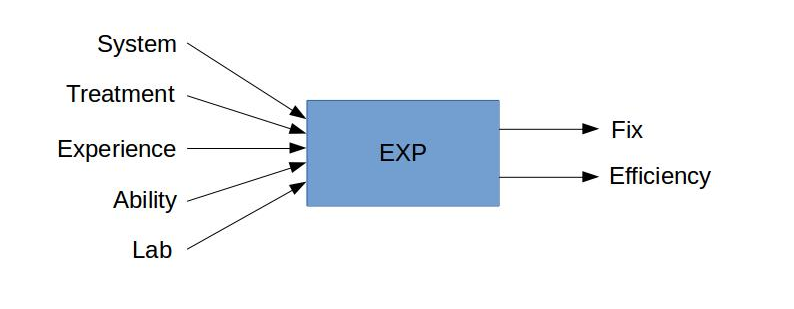
\includegraphics[ width=1 \linewidth]{./img/GLM_debugging.png}
	 As can be seen from the image the GLM considers parameters listed above and provides an estimation about Effectiveness (number of correctly fixed bugs) and Efficiency (time requested to fix a bug).
	 
\subsection{Script} \newpage
\begin{lstlisting}[language=R]
data = read.csv2("all.csv", sep=";", dec=",", header=TRUE)

# Delete useless rows
selected = data[,c("ID", "Experiment", "Group", "System", "Treatment", "Lab", "Experience", "Ability", "Time1", "Fix1", "Time2", "Fix2", "Time3", "Fix3", "Time4", "Fix4")]

# Selecting only "All" rows
all = selected[selected$Experiment == "All",]

# Generate the column "Fix"
sumna = function(a) sum(a, na.rm=TRUE)
all = cbind(all, apply(all[,c("Fix1", "Fix2", "Fix3", "Fix4")], 1, sumna)) 
colnames(all)[length(all)] = "Fix"

# Calculate efficiency, NA and NaN are converted to 0.
efficiency = function(a) if (a[9] != 0 )a[9]/sumna(c(a[1]*a[2], a[3], a[4], a[5]*a[6], a[7]*a[8])) else 0
alleff = cbind(all, apply(all[,c("Time1", "Fix1", "Time2", "Fix2", "Time3", "Fix3", "Time4", "Fix4", "Fix")], 1, efficiency)) 
colnames(alleff)[length(alleff)] = "Efficiency"

attach(alleff)
#Rename litteral data to integers 
abLevel = function(l) if(l == "low") 1 else if(l == "medium") 2 else if(l == "high") 3
Ability = sapply(alleff$Ability, abLevel)

#GLM
fixModel = glm(Fix ~ System + Treatment + Lab + Experience + Ability)
effModel = glm(Efficiency ~ System + Treatment + Lab + Experience + Ability)

#Draw effectiveness plots
boxplot(Fix ~ Ability, names=c("Low", "Medium", "High"), xlab="Ability", ylab="Effectiveness")
boxplot(Fix ~ Treatment, xlab="Treatment", ylab="Effectiveness")
interaction.plot(Treatment, alleff$Ability , Fix, trace.label = "Ability")

#Draw efficiency plot
interaction.plot(Treatment, Ability, names=c("Low", "Medium", "High"), Efficiency)
interaction.plot(Treatment, alleff$Ability , Efficiency)
interaction.plot(Treatment, alleff$Ability , Efficiency, trace.label = "Ability")

detach(allef)

\end{lstlisting}
	
\newpage
	\subsection{Effectiveness Results}
This is the raw data output of the effectiveness experiment's GLM.
\begin{lstlisting}[language=]
Call:
glm(formula = Fix ~ System + Treatment + Lab + Experience + Ability)

Deviance Residuals: 
 Min       1Q   Median       3Q      Max  
-1.5491  -0.7680  -0.2572   0.9079   2.2216  

Coefficients:
                Estimate Std. Error t value Pr(>|t|)    
(Intercept)         -1.3959     0.5404  -2.583 0.013195 *  
Systemxml-security  -0.2230     0.3050  -0.731 0.468539    
Treatmentrandom      0.6964     0.3036   2.294 0.026621 *  
Lablab2              0.2858     0.3126   0.914 0.365525    
Experiencemsc        0.7706     0.3193   2.413 0.020035 *  
Ability              0.9443     0.2579   3.661 0.000671 ***
---
Signif. codes:  0 ‘***’ 0.001 ‘**’ 0.01 ‘*’ 0.05 ‘.’ 0.1 ‘ ’ 1

(Dispersion parameter for gaussian family taken to be 1.133588)

 Null deviance: 93.380  on 49  degrees of freedom
Residual deviance: 49.878  on 44  degrees of freedom
AIC: 155.77

Number of Fisher Scoring iterations: 2
\end{lstlisting}

\begin{figure}
		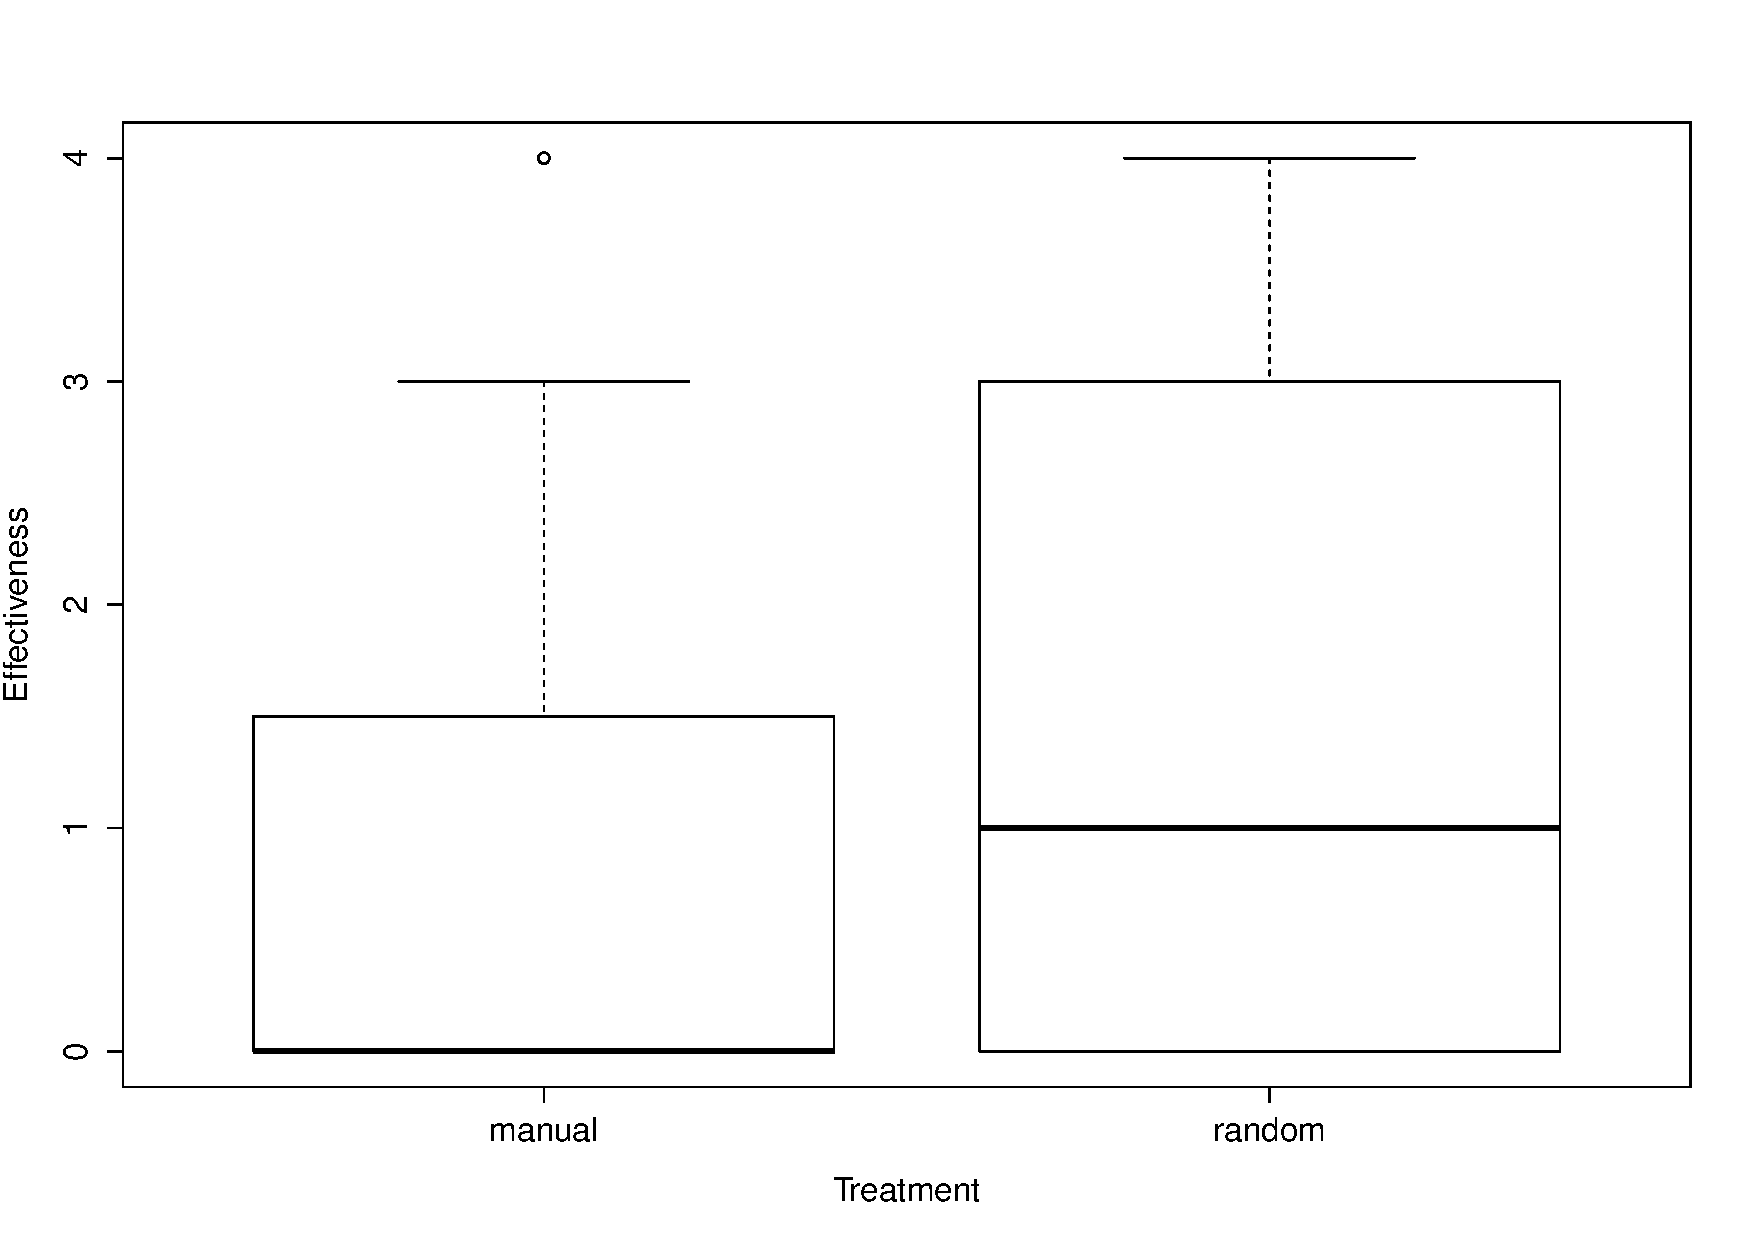
\includegraphics[ width=0.5 \linewidth]{./img/box_fix_treatment.pdf}
		\caption{Fix-Treatment Boxplot}
		\label{box_fix_treatment}
	\end{figure}

\begin{figure}
	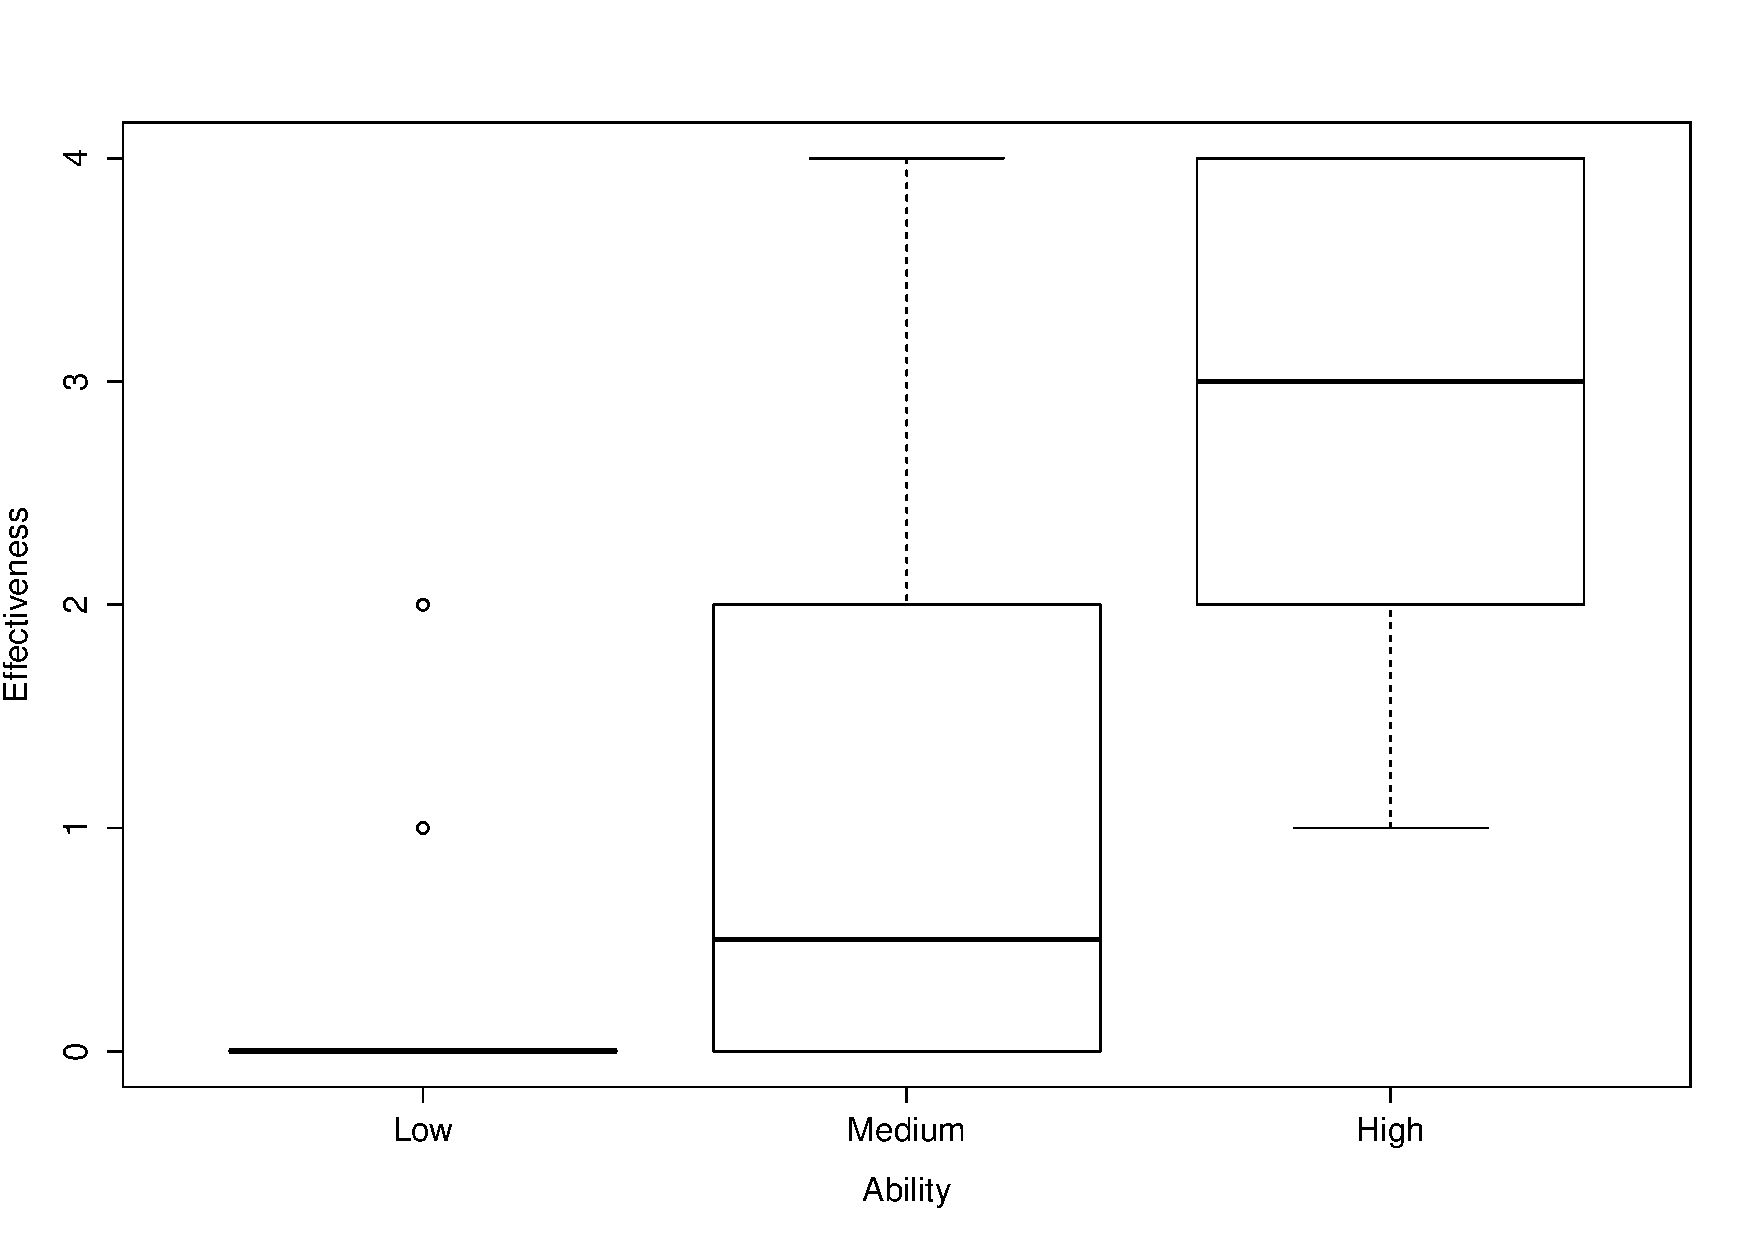
\includegraphics[ width=0.5 \linewidth]{./img/box_fix_ability.pdf}
	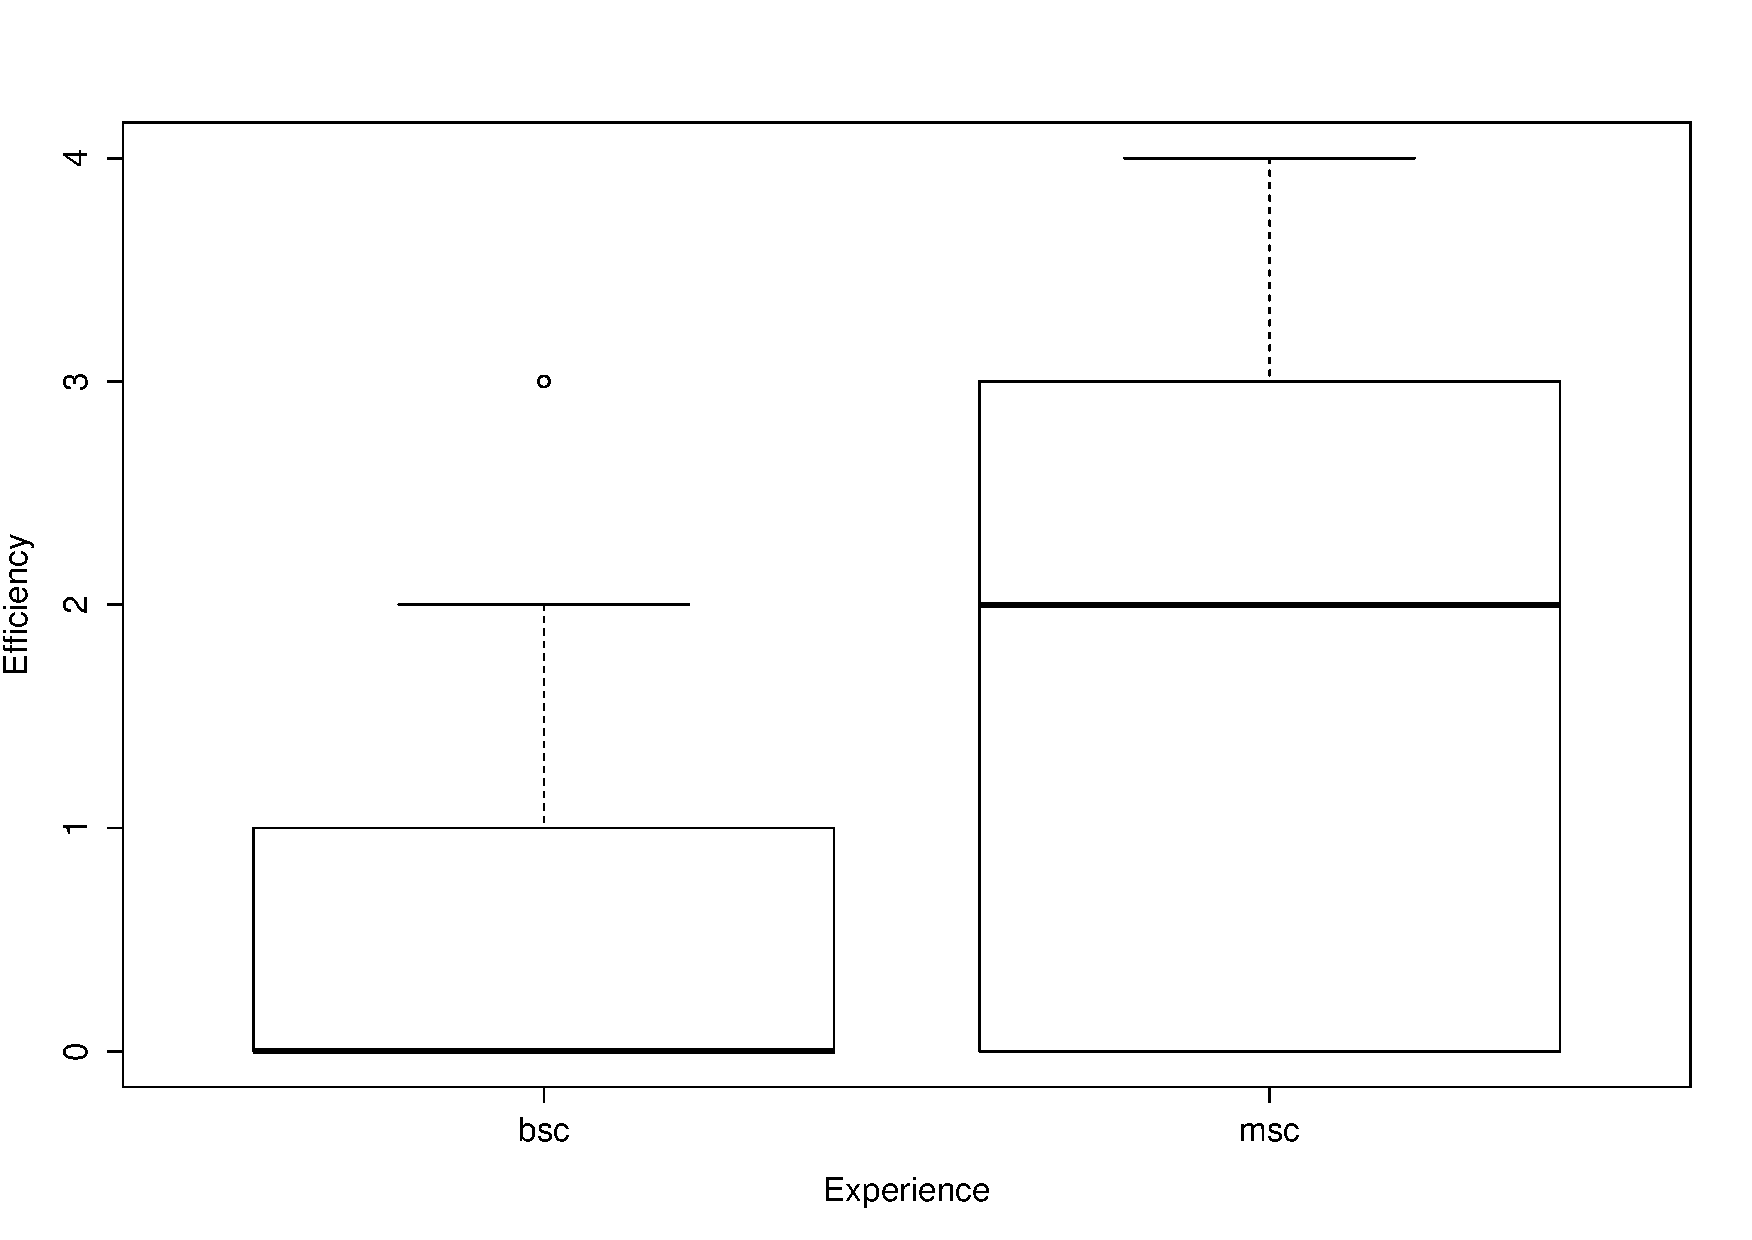
\includegraphics[ width=0.5 \linewidth]{./img/box_fix_experience.pdf}
	\caption{Effectiveness respect to Ability and experience Boxplots}
	\label{box_fix_ability}
\end{figure}

\begin{figure}
	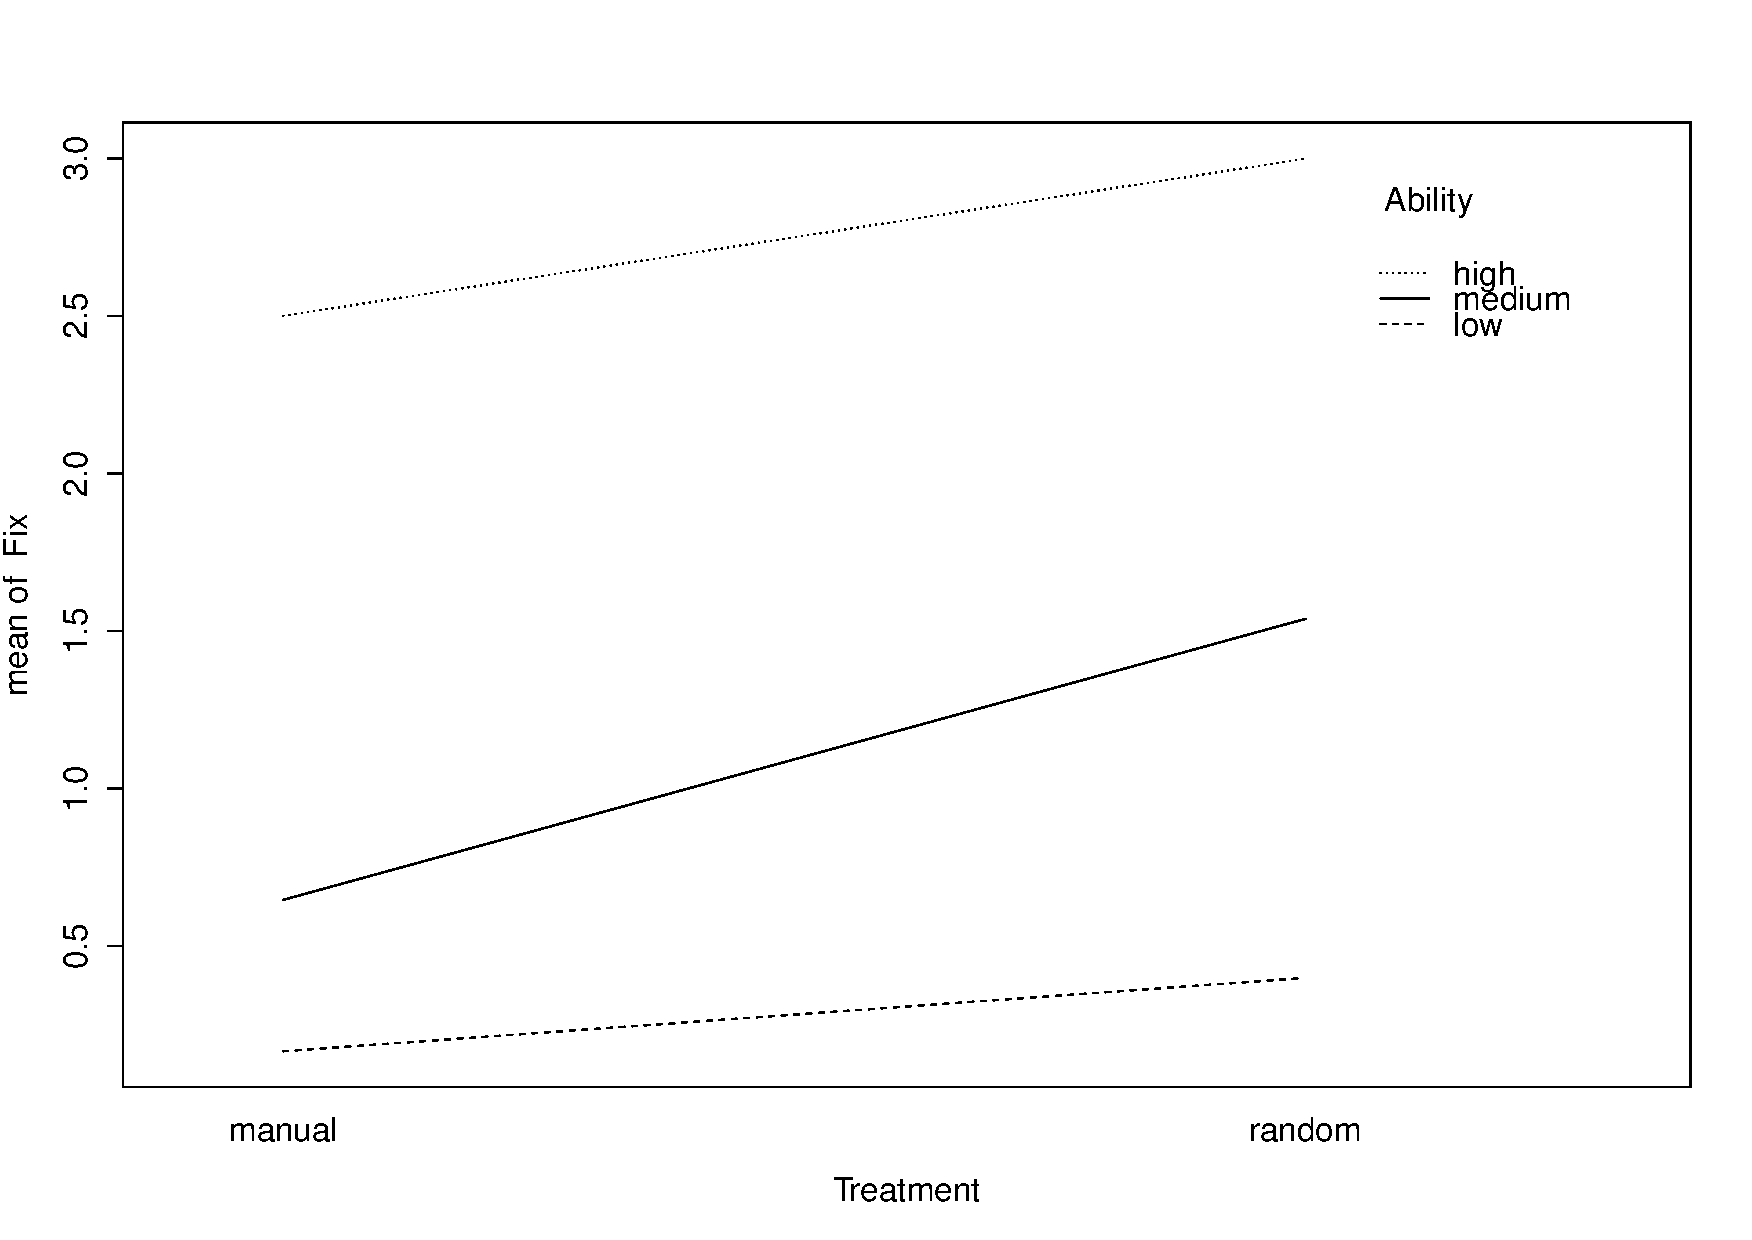
\includegraphics[ width=1 \linewidth]{./img/interaction_FixTreatmentAbility.pdf}
	\caption{Treatment, Effectiveness and Ability Interaction plot}
	\label{int_fix}
\end{figure}

Report conclusion about effectiveness can be summarized in the following quotation:
\begin{quote}
	\begin{itemize}
	\itembf{Treatment:} We can observe that subjects who used autogen tests showed better effectiveness (i.e., correctly fixed more faults) than subjects who used manually written tests.
	
	\itembf{Ability:} We can notice that the high ability and high experience subjects are associated with a line substantially higher than the line for the low ability/experience subjects
	
	\itembf{Experience:} high experience subjects improve their performance when using autogen tests much more than lower experience subjects do. In other words, subjects with high experience are better at taking advantage of the higher effectiveness provided by autogen tests.
	
	\itembf{System and Lab:} we can notice that System and Lab are not significant factors, thus there is no effect
	of the system and no learning effect between the two experimental sessions.
	TREATEMENT: We can observe that subjects who used autogen tests showed better effectiveness (i.e., correctly fixed more faults) than subjects who used manually written tests.

	\end{itemize}
\end{quote}
Accordingly with results we can observe from R output that Efficiency is significantly influenced by Treatment (confidence at 95 \%), Experience (confidence at 95 \%) and Ability (confidence over 99 \%). Session and the System used do not influence Effectiveness in a significant measure. Observing the figure \ref{int_fix} can be seen that all programmers perform better with random test cases, in particular those with medium or higher experience and this is confirmed also from figure \ref{box_fix_treatment}.\\
Experience is also important as can be seen both from figure  \ref{box_fix_ability} and \ref{int_fix}

\subsubsection{Formula}
\begin{equation}
\begin{split}
	\hat{Fix} = f(Tr, Ex, Ab) = A_{1}*Tr + A_{2}*Ex + A_{3}*Ab + A_{0} \\
	\hat{Fix} = f(Tr, Ex, Ab) = 0.696*Tr + 0.77*Ex + 0.944*Ab + -1.396
\end{split}
\end{equation}

% % % % % % % % % % % % % % % % % % % % % % % % % % % % % % % % % % % % % % % % % % % % % % % % % % % % % % % % % % % % % % % % % % % % % % % % % % % % % % % % % % % % % % % % % % % % % % % % % % % % % % % % %
\newpage
\subsection{Efficiency Results}
This is the raw data output of the efficiency experiment's GLM.
\begin{lstlisting}[language=]
Call:
glm(formula = Efficiency ~ System + Treatment + Lab + Experience + 
    Ability)

Deviance Residuals: 
      Min         1Q     Median         3Q        Max  
-0.061021  -0.021901  -0.009289   0.017966   0.203006  

Coefficients:
                     Estimate Std. Error t value Pr(>|t|)    
(Intercept)        -0.0784003  0.0232811  -3.368  0.00158 ** 
Systemxml-security -0.0103287  0.0131413  -0.786  0.43610    
Treatmentrandom     0.0408678  0.0130782   3.125  0.00315 ** 
Lablab2             0.0005354  0.0134652   0.040  0.96847    
Experiencemsc       0.0208320  0.0137561   1.514  0.13708    
Ability             0.0490092  0.0111127   4.410 6.57e-05 ***
---
Signif. codes:  0 ‘***’ 0.001 ‘**’ 0.01 ‘*’ 0.05 ‘.’ 0.1 ‘ ’ 1

(Dispersion parameter for gaussian family taken to be 0.002103959)

    Null deviance: 0.183689  on 49  degrees of freedom
Residual deviance: 0.092574  on 44  degrees of freedom
AIC: -158.69

Number of Fisher Scoring iterations: 2
\end{lstlisting}

\begin{figure}
		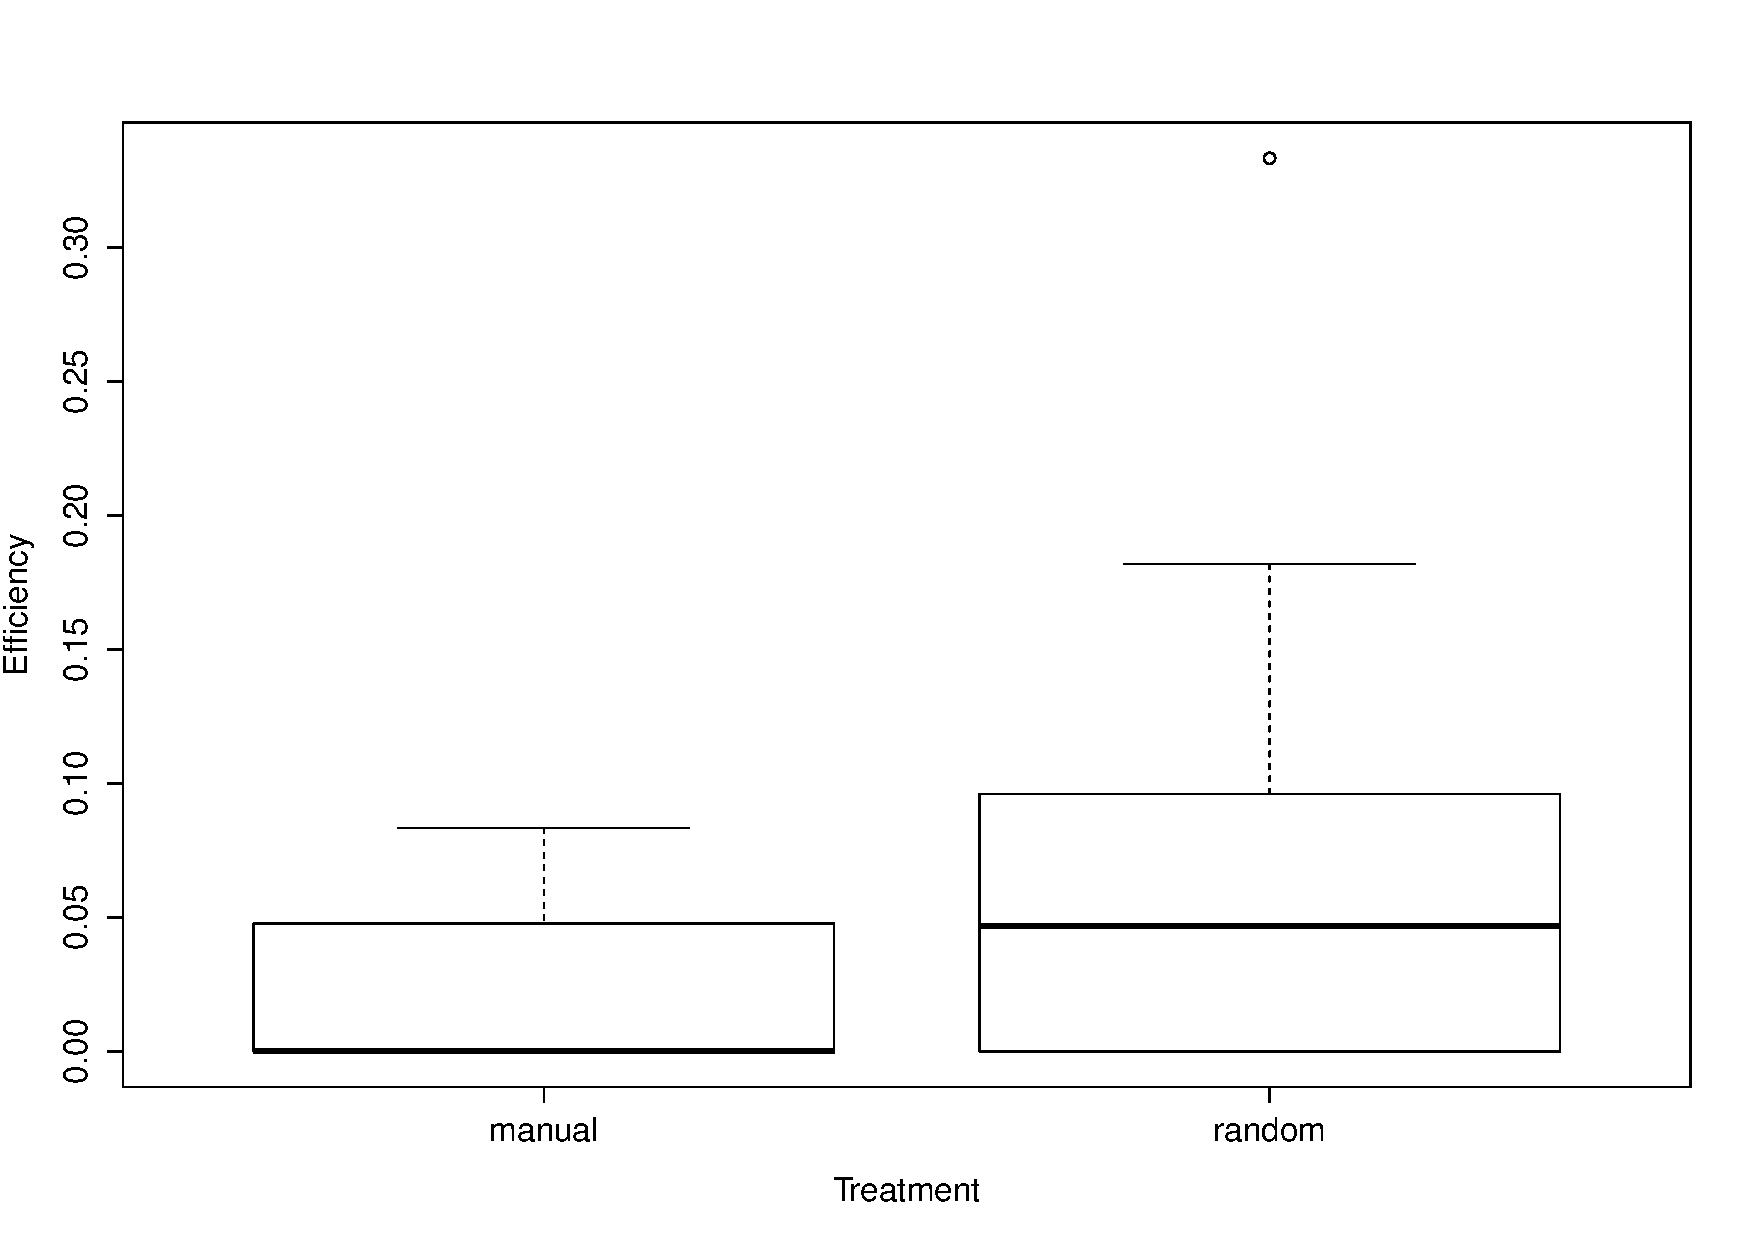
\includegraphics[ width=0.5 \linewidth]{./img/box_eff_treatment.pdf}
		\caption{Efficiency-Treatment Boxplot}
		\label{box_eff_treatment}\begin{equation}
		\begin{split}
			\hat{Fix} = f(Tr, Ex, Ab) = A_{1}*Tr + A_{2}*Ex + A_{3}*Ab + A_{0} \\
			\hat{Fix} = f(Tr, Ex, Ab) = 0.696*Tr + 0.77*Ex + 0.944*Ab + -1.396
		\end{split}
		\end{equation}
	\end{figure}

\begin{figure}
	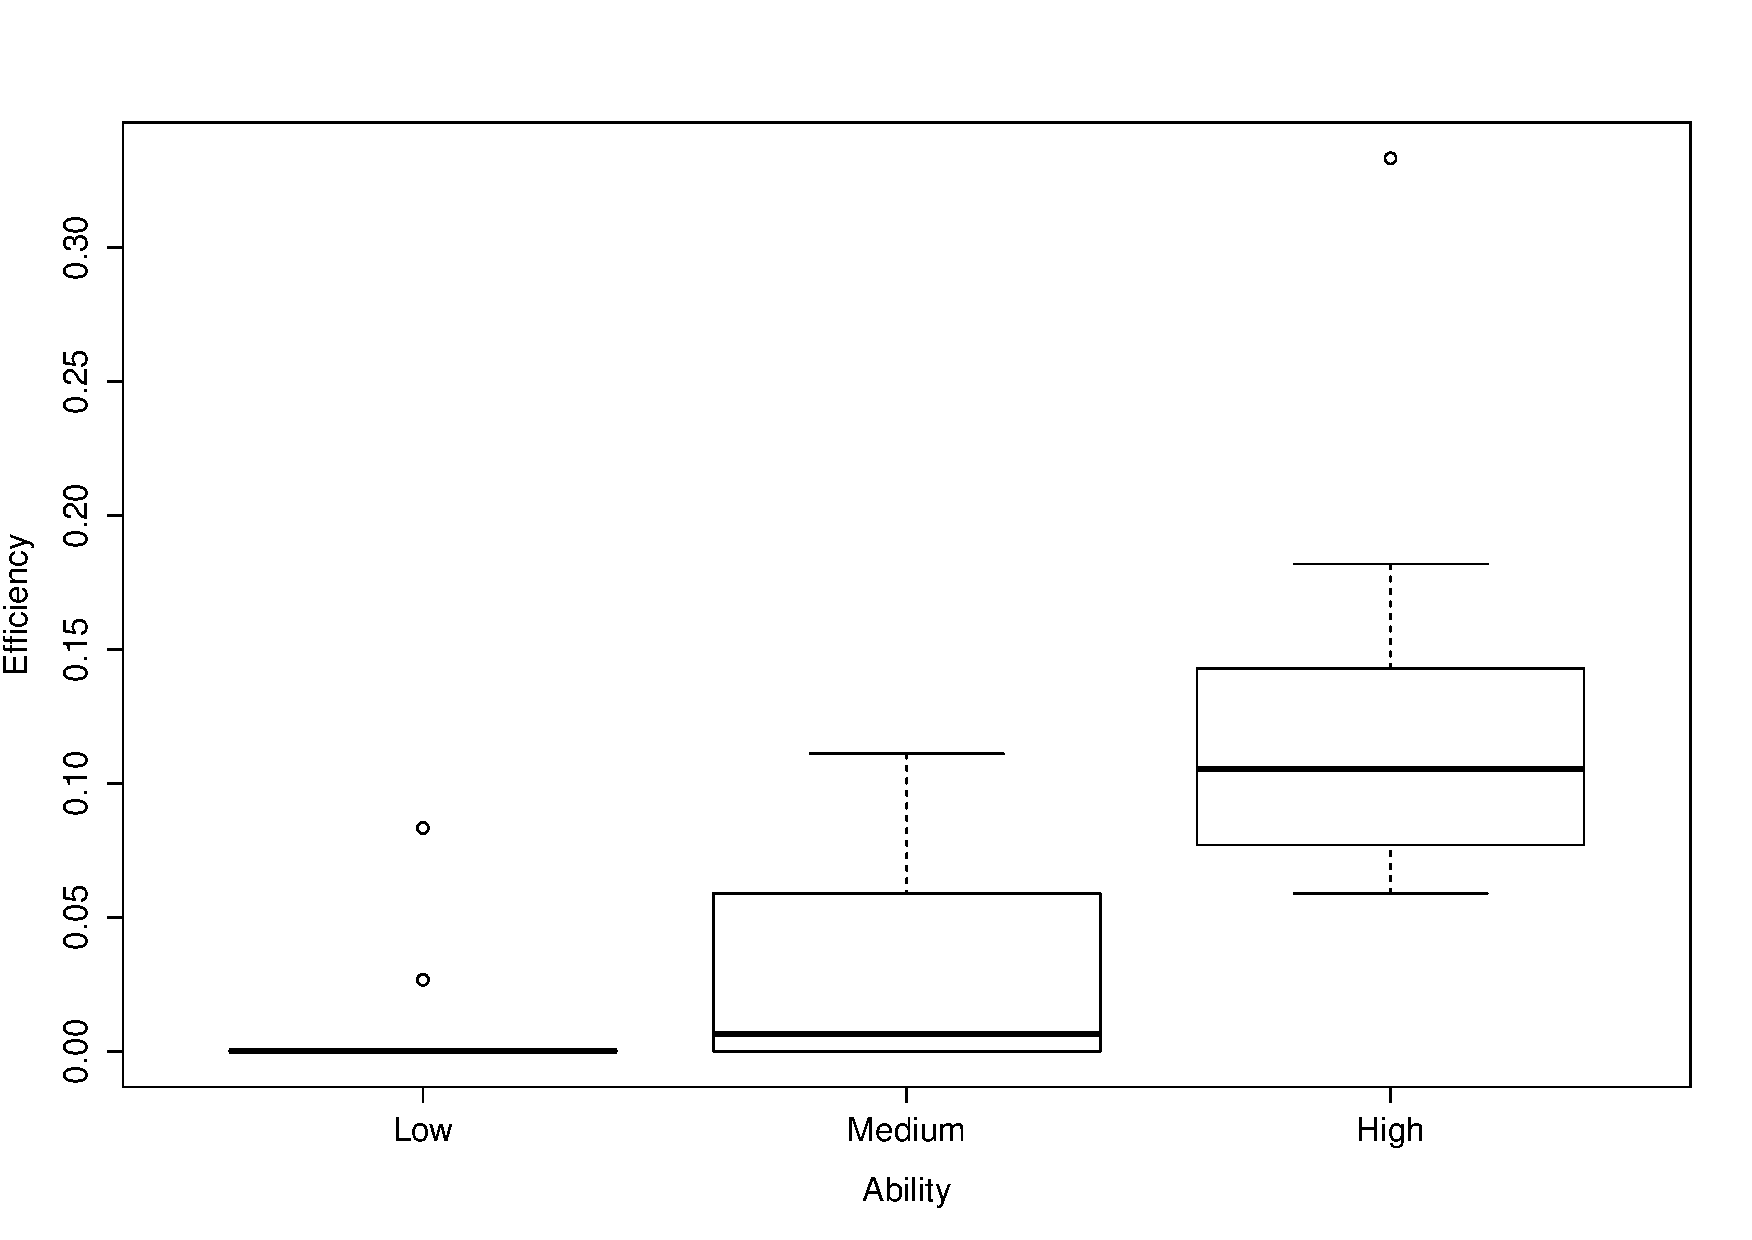
\includegraphics[ width=0.5 \linewidth]{./img/box_eff_ability.pdf}
	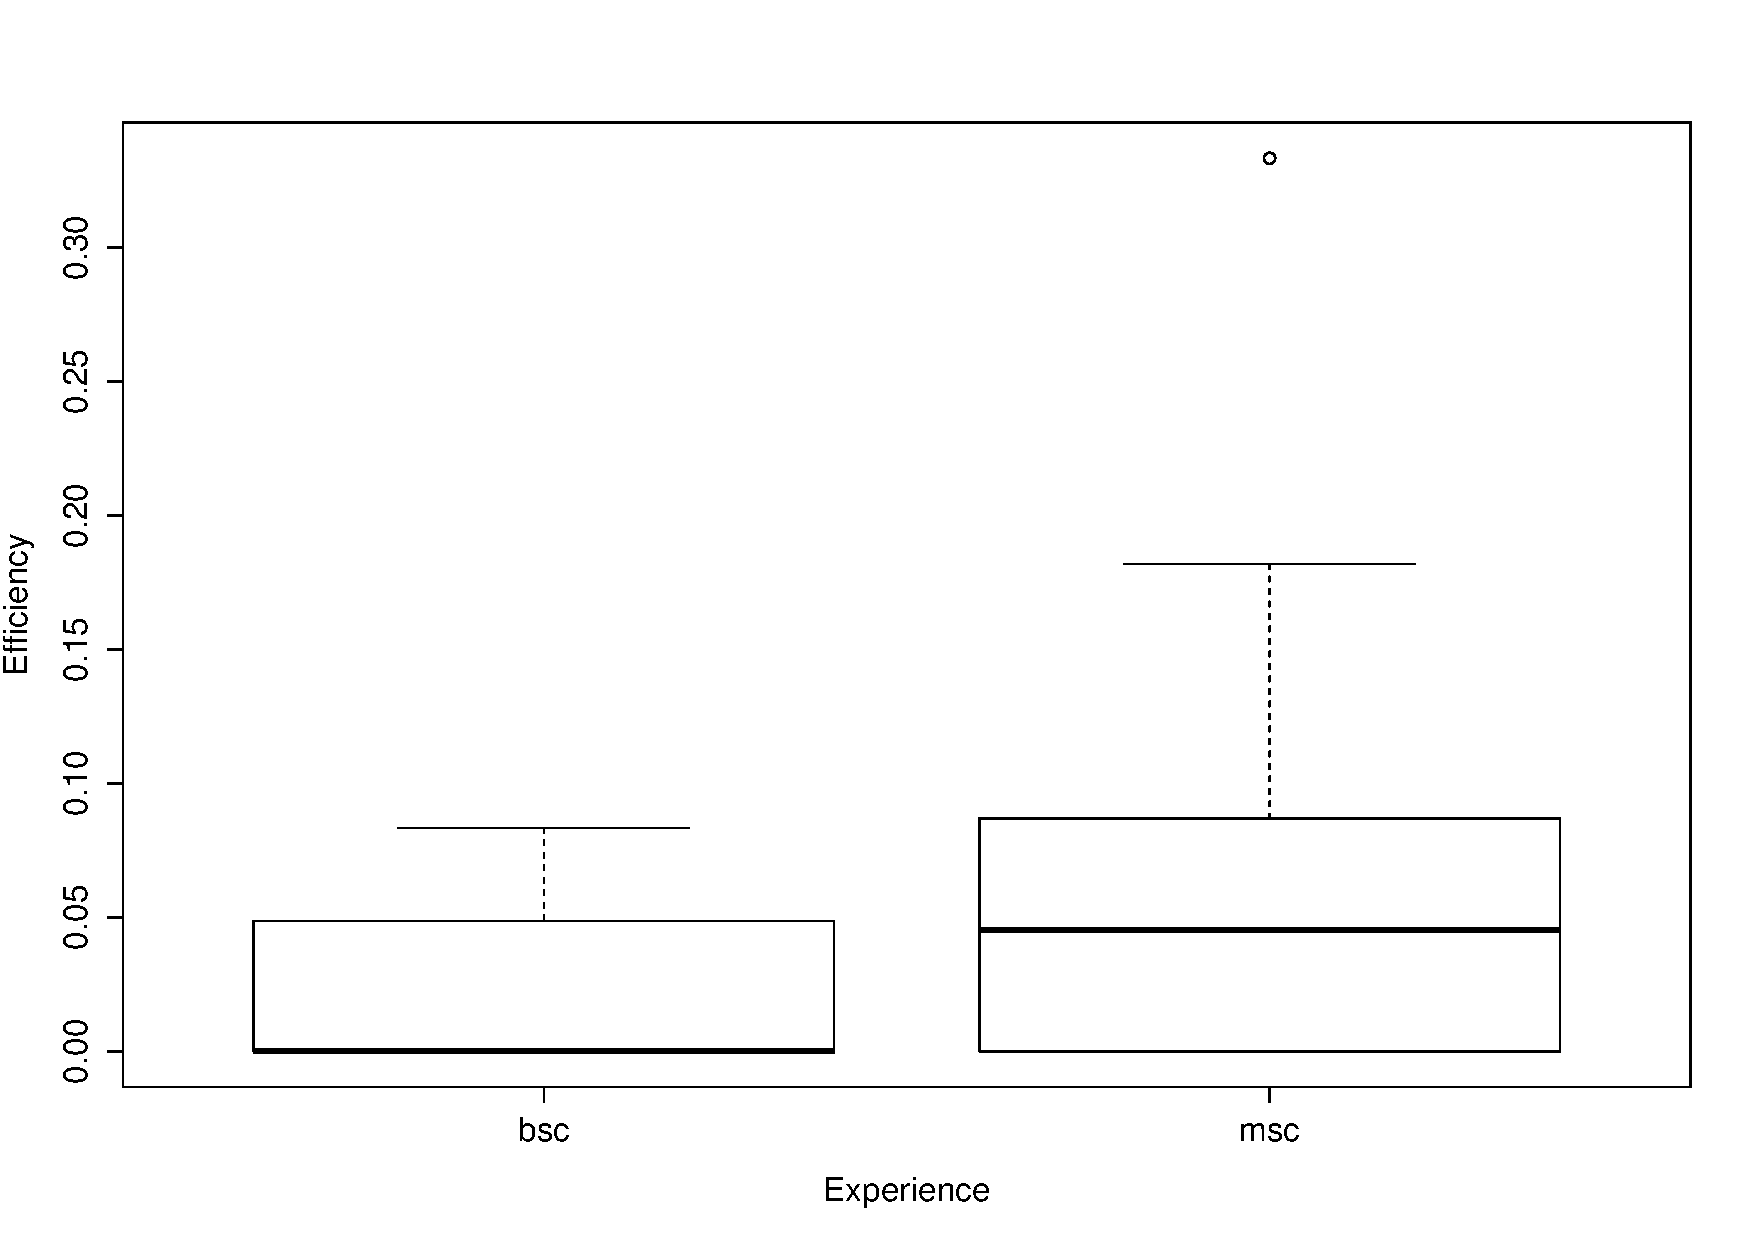
\includegraphics[ width=0.5 \linewidth]{./img/box_eff_experience.pdf}
	\caption{Efficiency respect to Ability and experience Boxplots}
	\label{box_eff_ability}
\end{figure}

\begin{figure}
	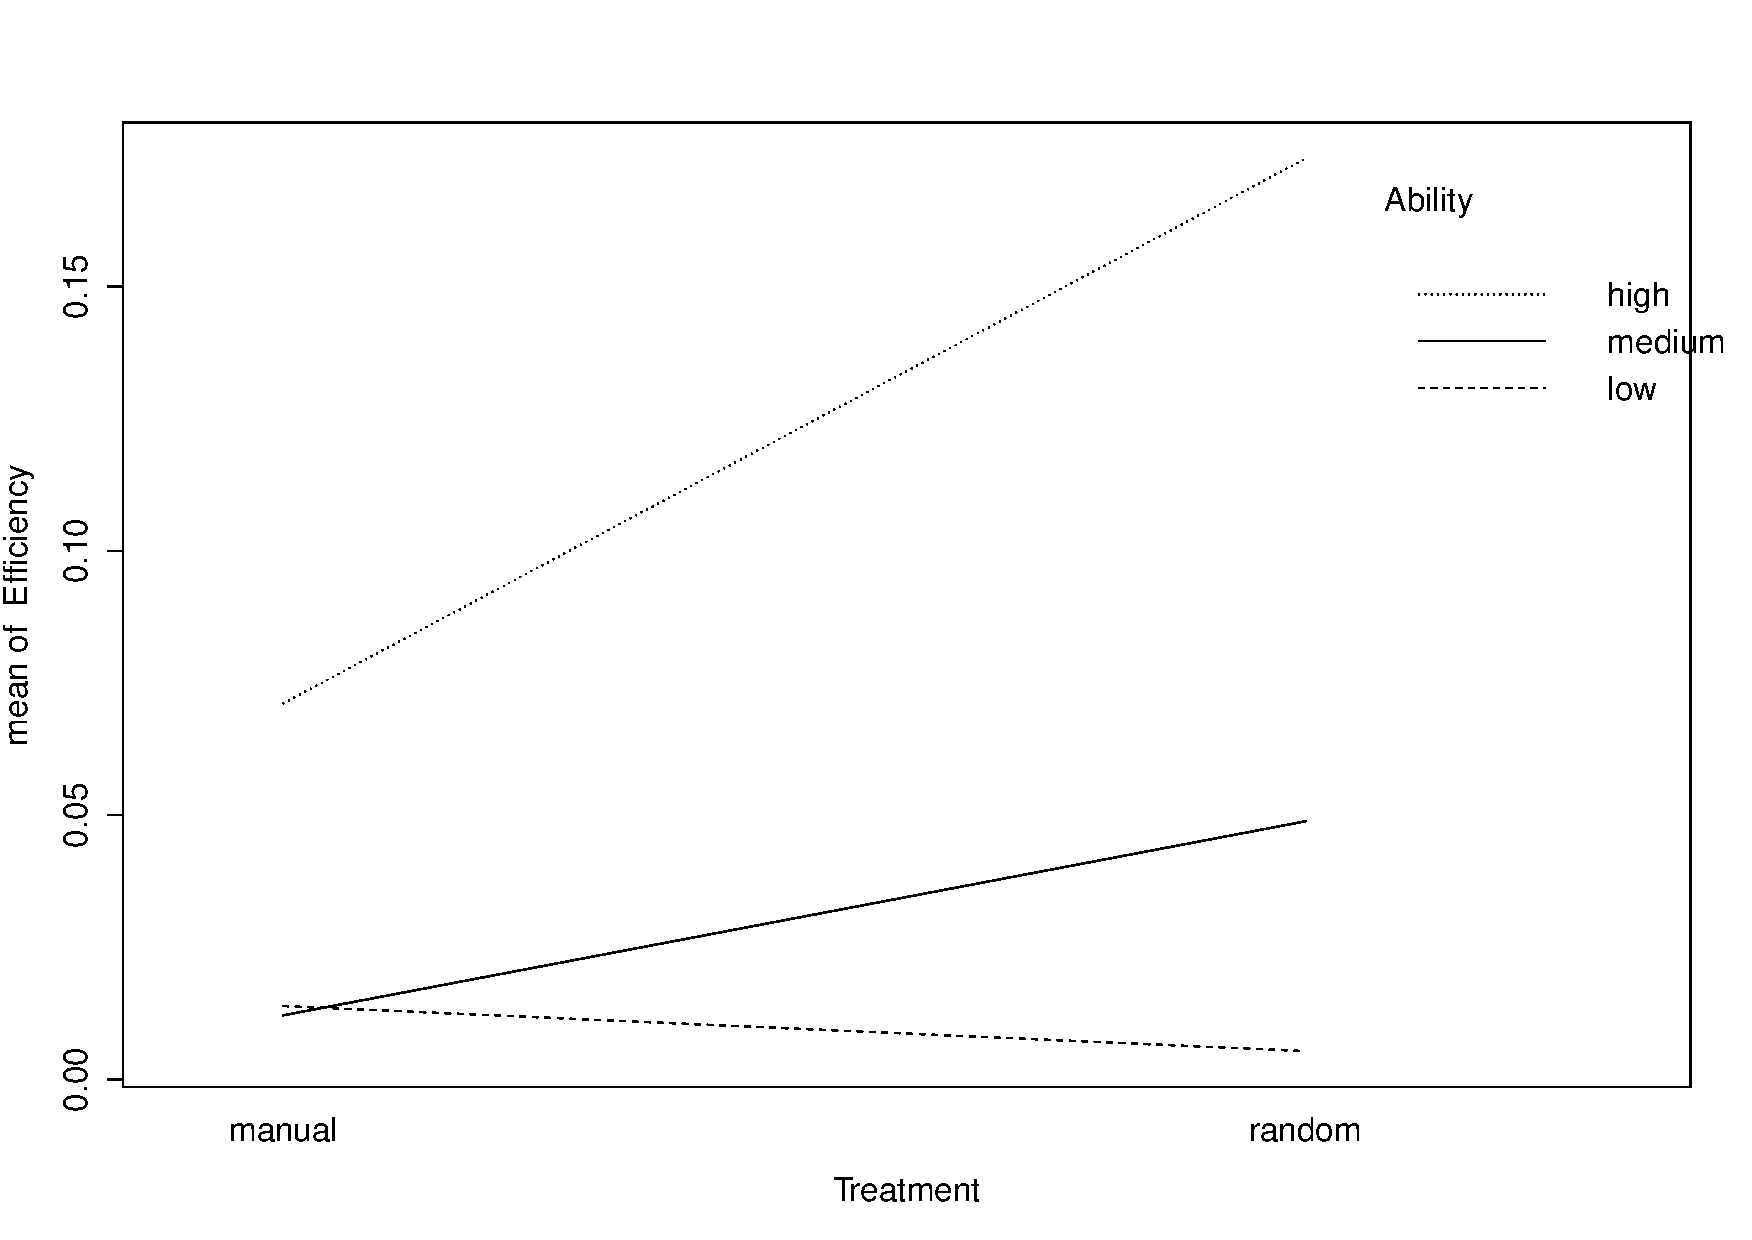
\includegraphics[ width=1 \linewidth]{./img/interaction_EfficiencyTreatmentAbility.pdf}
	\caption{Treatment, Efficiency and Ability Interaction plot}
	\label{int_eff}
\end{figure}

Report conclusion about effectiveness can be summarized in the following quotation:
\begin{quote}
	\begin{itemize}
	\itembf{Treatment:} The efficiency of subjects working with autogen tests is higher than when working with manually	written tests.  
	
	\itembf{Ability and Experience:} Higher ability/experience subjects are particularly	good at taking advantage of the higher efficiency associated with the use of autogen tests.
	
	\itembf{System and Lab:} Factors System and Lab do not have a significant influence on efficiency of debugging.
	of the system and no learning effect between the two experimental sessions.

	\end{itemize}
\end{quote}
Accordingly with results we can observe from R output that Efficiency is significantly influenced by Treatment (confidence at 99 \%) and Ability (confidence over 99 \%). Nor experience neither Session and the System used influence Efficiency in a significant measure.\\
Observing the figure \ref{int_eff} can be seen that programmers with medium or higher experience performs significantly better with random test while lesser experienced developers performs better with manual test. This strange behavior can be explained looking at data table: most data involving low-ability programmers are corrupted and only two cases are significant, all other rows report a fix and efficiency equal to 0 because of several missing data. This probably also influence Experience result: most low-ability subjects are also bsc.

\subsubsection{Formula}
\begin{equation}
\begin{split}
	\hat{Eff} = f(Tr, Ab) = A_{1}*Tr + A_{2}*Ab + A_{0} \\
	\hat{Eff} = f(Tr, Ab) = 0.04*Tr + 0.049*Ab + -0.078
\end{split}
\end{equation}

\chapter{CodeSurfer}

\section{Usage}
CodeSurfer performs deep semantic analysis on the given code allowing the develper to understand how exactly the program works. It provides only valid executions.
Paths can be explored through a GUI and are and can be influenced by dependences (inter-variable assignments) including pointers, and allows automatic queries to resolve variables relationship. \cite{csurfUserGuide2012}

\begin{itemize}
	\itembf{String Constant Pointer Targets} (one-string/many-strings): differences in strings can be ignored (e.g. can be useful when analyzing GUI code) , or considered as different 
	\itembf{Variable Use/Def Sets} (yes/no): distinguish or not conditional kills 
	\itembf{Compute GMOD}(yes/no): determine dependences on non-local variables, this function is time-consuming
	\itembf{Compute Data Dependence}(yes/no): compute data dependency 
	\itembf{Compute Control Dependence} (yes/no):compute call dependecy, is only space consuming
	\itembf{Compute Summary Edges}(yes/no): is space and time consuming, it affects the interprocedural precision of slicing and chopping
	\itembf{Control Flow Edges}(yes/both/no): can compute CF edges, directed edges or none. The procedure is very cheap.
\end{itemize}

CodeSurefer can be run with 5 presets (super-lite, lite, medium, high and highest) they respectively enaable: nothing expensive, CFG only, no DD and imprecise pointer analysis, no context sensitive and string and fields are represented as scalar, finally no limitation is enforced. Lite and super-lite are intended as a check before the usage of a more precise execution.

\subsection{C++ Tutorial}
\subsubsection{Build a project}
Csurf gets a source code as input and build it generating a project that will be opened in the GUI. A project name, a compiler (or make if a makeFile is available) and a target has to be specified.
\begin{lstlisting}[language=bash]
csurf hook-start <projectName> <compiler> <target>

csurf hook-start hello cc hello.c

#WARN: instructions above will build the project with the lowest preset which does not allow some kind of analysis! To specify another level (e.g. highest) use command below:

csurf hook-start <projectName> -preset-build-options highest --- make  <target>
\end{lstlisting}

\subsubsection{Surfing a project}
A project can be opened using the project name without any extension.
\begin{lstlisting}
csurf <projectName>
\end{lstlisting}
clicking on the "source.c" element the code structure can be explored. CodeSurfer generates several functions such as \#zFile\_Initialization \#Global\_Initialization\_i (where i is a number).


\subsubsection{Queries}
The deep structure of a project is represented as a directed graph of program points connected by dependence edges. There are two main methods to calculate the dependes of a piece of code from the others:
\begin{itemize}
	\itembf{Data Dependeces:} is based on the assignment of values, a variables depends on others whose are involved in the calculation of its value. E.g. $x = y + z$ where x depends both on y and z.
	\itembf{Control Dependences:} the analysis is based on the control flow of the program (loops, conditions etc...), in this case the value of a variable depends on the variable present in the condition e.g. $if (x < 1) then (y = z) else (y = 0)$ in this case y depends on x.
\end{itemize}
Usually both CD and DD analysis are performed because the real value of a variable depends both on control flow and assignaments. In particular cases, to save resources, only one of the two analysis can be performed. In any case the result is not a final value but a flow graph which includes all variable dependences.\\
A Criterion is define as the combination of a point (a statement, line of code) and a specific variable, however CodeSurfer allows the usage of only the variable or the statment to define a criterion.
\\\\
CodeSurfer assumes that every loop may execute zero times, even when the program is simple enough to tell otherwise. In some contexts, all dependences are classified as either control or data dependences. In such contexts, declaration dependences are treated as data dependences.

\begin{itemize}
	\itembf{Predecessor/Successor:} starts from some query-points, pred/succ can be calculated DD and/or CD
	\itembf{BackWard/Forward Slicing:} the program is analyzed using CD and DD startring from the specified point and finding all the variables which contributes to the selected variable (Backward)or all the variables which the selected variable contributes to (Forward). Expanding the source file and clicking on a specific function Slicing can be applied: all reachable functions are coloured red, unreachable black. CodeSurfer typically errs on the safe side, creating false positives rather than missing effects that may be important.
	\itembf{Chop:} two points (chop-source and chop-target), the procedu is similar to the intersection of forward and backward slicing, the graph involves all operations that lead from the source to the targes. Source and target can be sets of points. 
\end{itemize}

The analysis of a program which involves functions is slightly complicated: suppose to have a function $int f(x)$ which is called in two points of the main(). When the function is called the main program stops esecutin, pass a value to f which returns a value, then the main restart executing. Analizing a code which calls two times the same function the resulting graph will have two edges from main to f and two edges from f to main. Obviously use the first main-to-f and the second f-to-main makes no sense and those spurious path have to be ignored.

%%%%%%%%%%%%%%%%%%%%%%%%%%%%%%%%%%%%%%%%%%%%%%%%%%%%%%%%%%%%%%%%%%%%%%%%%%%%%%%%%%%

\section{Program Representation}
\subsection{Control Flow Graph}
A CFG is a graph wich represent the executions steps of a program, it has only and entry point (where the execution begins) and only one exit point (where the execution ends). If the program has more than one entry/exit points them are merged in a single bogous entry/exit point. Each function is represented as a sub-CFG with the same characteristics.
\subsubsection{Syntax}
Inter-procedural edges (function call and return) are represented with an horizontal dashed arrow, while intra-procedural (inside the same function) steps are represented using a solid arrow. A vertical dotted line represent intraprocedural execution while a function is executed (i.e. the execution in main between call f and return f).
\begin{itemize}
	\itembf{IF} statments have labeled branches (true/false), the two branches merge once complethed the different execution
	\itembf{LOOPS} for and while statments have labeled branches (true/false), the  true branch execute the loop and return to the condition, the false branch skip the condition and reach the external code
	\itembf{EXCEPTION} are handled using a normal-exit vertex and an exceptional-exit vertex, both reach the exit status
\end{itemize}

\subsection{System Dependence Graph}
An SDG is similar to a CFG: it has a single entry/exit point so has it's functions, each instruction is a node and each step is an edge.
In addition to inter/intra-procedural edges SDGs introduce the Control and Data Dependences as seen above. Inter and intra procedural calls are still represented using dashed and solid edges, while the CD and DD are distinguished changing the colour of the (solid or dashed) edge.\\
Data Dependences are calculated using forward slicing, i.e. as the current variable will influence next states.
\begin{figure}
	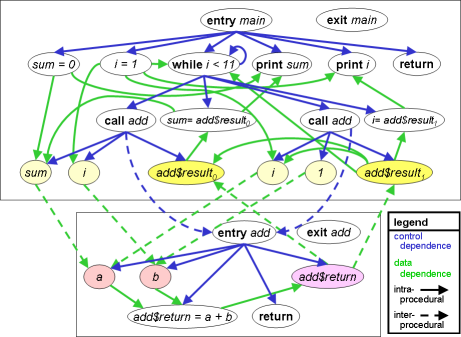
\includegraphics[ width=0.8 \linewidth]{./img/sdg_diagram.png}
	\caption{System Dependence Graph in CodeSurfer manual }
	\label{sdg_csurf}
\end{figure}



%%%%%%%%%%%%%%%%%%%%%%%%%%%%%%%%%%%%%%%%%%%%%%%%%%%%%%%%%%%%%%%%%%%%%%%%%%%%%%%%%%%

\section{Scheme}
Csurf can be extended both with c and shceme script. Scheme script can be run in batch mode and can access csur API in order to perform custum analisis. Those scripts can be run using 
\begin{lstlisting}
csurf -nogui -l <script.stk> <project>
\end{lstlisting}
Where nogui suppress the graphical interface and -l specify the script.
\\\\
Scheme is a functional language derived from Lisp, it is weakly typed and objects can be unlimited extended because the memory is managed internally.
\cite{abelson1991revised}
\subsection{Syntax}

Each expression has to be surrounded by parenthesis e.g. (display "hello world"), be aware that () are not intended like {} in C or Java but means something like "evaluate" as \$() does in bash. For this reason their number is relevant, for example (display "hello") is correct while ((display "hello")) is not!
Functions do not use the traditional parenthesized notation f(a, b) but are red in order from left to right where the first argument is the procedure (f a b). E.g. (a + b) is not valid, it has to be written as (+ a b)\\
Upper and lower case forms of a letter are never distin-guished except within character and string constants.\\

\subsubsection{Basic commands}
\begin{itemize}
	\itembf{;} comments are intruduced using ; and involves a single line
	\itembf{procedure?} conventionally are procedures which returns a boolean variable
	\itembf{procedure!} conventionally are procedures which write a result into a previously allocated memory location
	\itembf{"string"} strings are surrounded by "
	\itembf{lambda((args) (expr) values)} declares a procedure e.g. ((lambda (x y) (+ x y)) 3 4) returns 7 
	\itembf{define name (lambda)} without values associates a procedure to a name, it can be called using (name values)
	\itembf{let name ((var value))(expr)} is used to declare one or more variables which exists only inside the let scope, e.g. (let ((x 3) (y 4)) (+ x y)) returns 7. Nested let can hide variables declared in external scopes, on the contrary let* override the value of the external variable. The "name" parameter is optional: if it is specified the named let can be used like a local function.
	\itembf{cond(((test1)(inst1))((test2)(instr2)))} conditions are tested in succession, if one is satisfied the associated instruction is executed and following conditions are not tested. It basically works like a switch-case, the default condition can be simulated using (\#t (defaultop))
	\itembf{if (cond) (thenInstr)(elseInstr)} the condition is evaluated and, if it is satisfied, the first instruction has been executed, otherwise the second
	\itembf{set! var } 
\end{itemize}

\subsubsection{Reserved Keywords}
\begin{lstlisting} [language=lisp]
=>		do		or		and		else	quasiquote	begin	if		quote	case lambda	set!	cond	let		unquote	define	let*	unquote-splicing	delay	letrec
\end{lstlisting}

\subsubsection{Types}
	\begin{itemize}
		\itembf{Boolean} \#t \#f are the true and false values
		\itembf{Pairs} are represented with a dotted notation (a . b) that can be produced using the instruction (cons a b), car returns the first element, cdr the second. Be aware that cons (1 (list 2 3 4)) will return a list (1 2 3 4) and not a couple (1 . (2 3 4)) because is considered a special case of a list. In general the usage of cons should be avoided.
		\itembf{List} can be defined as a recursive applicarion of couples where the last element is null, for this reason car returns the first element and cdr the last one. a list can be declared using (list e1 e2 e3 ... en). Has some extra feture respect to pairs/nested pairs.
	\end{itemize}
	
\subsubsection{Constants}
	\begin{itemize}
		\itembf{'a} single quote, char value (a)
		\itembf{} backquote almost-constant data
		\itembf{"foo"} string, \ is the escape value
		\itembf{\#\textbackslash} character constants
		\itembf{\#()} vector constant
		\itembf{\#t \#f} boolean TRUE and FALSE
	\end{itemize}
	
\subsection{Function definition}
Basic function examples
\begin{lstlisting}[language=lisp]
;this function computes the sum of two elements
(define sum
	(lambda(a b)
		(+ a b)
	)
)

;this function compute recursively the factorial
(define fact
	(lambda(n)
		(if (= n 0)
			1						; base case "then"
			(* n (fact (- n 1)))	; recursion "else"
		)))
\end{lstlisting}

\subsection{Let}
Nested Let example
\begin{lstlisting}
; Nested Let
(define (myf vertex)
	(if (> vertex 0)
		(let ((x 12)(z 10))
			(let ((y (+ z 3)))
				(av-displayln  (+ x z))		
			)
		)
	)
)
\end{lstlisting}

\newpage
\subsection{List operation}
List declaration
\begin{lstlisting}[language=lisp]
; Empty list
(define lst (list))

(define lst (list 1 2 3 4 ))

; Equivalent to above
; Last element HAS to be empty otherwise a pair (list.element) will be generated!
(define lst (cons 1 (cons 2 (cons 3 (cons 4 '())))))
\end{lstlisting}

Some useful list operation
\begin{itemize}
	\itembf{(append list1 list2)} concatenation, both element has to be list eventually empty (list ) or of lenth 1 (list elm).
	\itembf{(member element list)} say whether or not an element belongs to the list return return the cdr of the list from the element on if true, false otherwise
	\itembf{(reverse lst)} reverse the list
	\itembf{(length lst)} returns the lenght of the list
	\itembf{(list-tail lst k)} which returns all elements except the fist k 
	\itembf{(list-ref list k)} which return the kth element
	\itembf{(null? element)} return true is a list is empty
\end{itemize}

Sum all the elements of a list without using lambda on the contrary of the previous example. 
\begin{lstlisting}[language=lisp]
(define (vsum1 lst) 
	(
		if(< (length lst)  1)
			0
			(+ (car lst) (vsum (cdr lst)))
	)	
)
\end{lstlisting}

Implementation of the built-in function reverse. Note that append requires list arguments otherwise will fail. The same function implemented using \textit{cons} will build a serie of nested couples which are NOT equivalent to the reversed list: length cannot be applied and cdr will return only the last elements because the first element is a couple of couple (of couple...).
\begin{lstlisting}[language=lisp]
(define (rev lst)
	(if (null? lst)
			'()
			(append(rev (cdr lst)) (list (car lst)))
	))
\end{lstlisting}

\subsection{File operations}
The following code open a port to read the file "myfile.txt" and pass it to readFile. This function read the file char by char through a named let (loop is a mere label) which works like a recursive function loop(x). This workaround in required beacause each read-char moves the read pointer a char ahead so the usage of ()display read-char) will print only a character every two.
\begin{lstlisting}
(define (readFile input)
	(let loop ((x (read-char input)))
		(if (not (eof-object? x))
		(begin
			(display x)
			(loop (read-char input))
		))))

(call-with-input-file "myfile.txt" readFile)
\end{lstlisting}

A simpler way to convert a file into a string is the following:
\begin{lstlisting}
	(define str (port->string port))
	(display str)
\end{lstlisting}

The output is simpler:
\begin{lstlisting}
(define (printFile output)
	(display "hello, world" output)
)

(call-with-output-file "myout.txt" printFile)
\end{lstlisting}

\section{CodeSurfer Data Structure}
In Scheme API each program is organized in a tree-like structure:
\begin{itemize}
	\itembf{SDG} System Dependence Graph, is composed by PDGs. An SDG represent the whole structure of a program including all methods.
	\itembf{PDG} Procedure Dependence Graph, is composed by Vertexes and Edges. A PDG represents a single procedure structure, it can belongs to several kind: user-defined (standard user-written functions), library and several kind of system defined (...-initialization) usually identified by a \# before their name.
	\itembf{Vertex} correspond to a program point, i.e. a combination of statement and line of code. Also vertexes are distinguised by kind, more intresting are entry/exit which represent the beginning and the end of a function, and call-site which identify a call to a function. Other Kind represent for example arguments, expression etc...
	\itembf{Edge} connect two vertexes, can be both intra-procedural (within the same PDG) and inter-procedural (between different PDGs). An edge is constituited by a vertex, which represent its target, and a label.
\end{itemize}

In \ref{csurf_uml} can be seen a partial representation of the Code Surfer class diagram. Only most significative functions and classes have been included in this representation. Note that Scheme is not an object-oriented language: several functions have been represented using the "object.function()" which has to be interpreted as a function which gets the object itself i.e. "(function object)".
\begin{figure}
	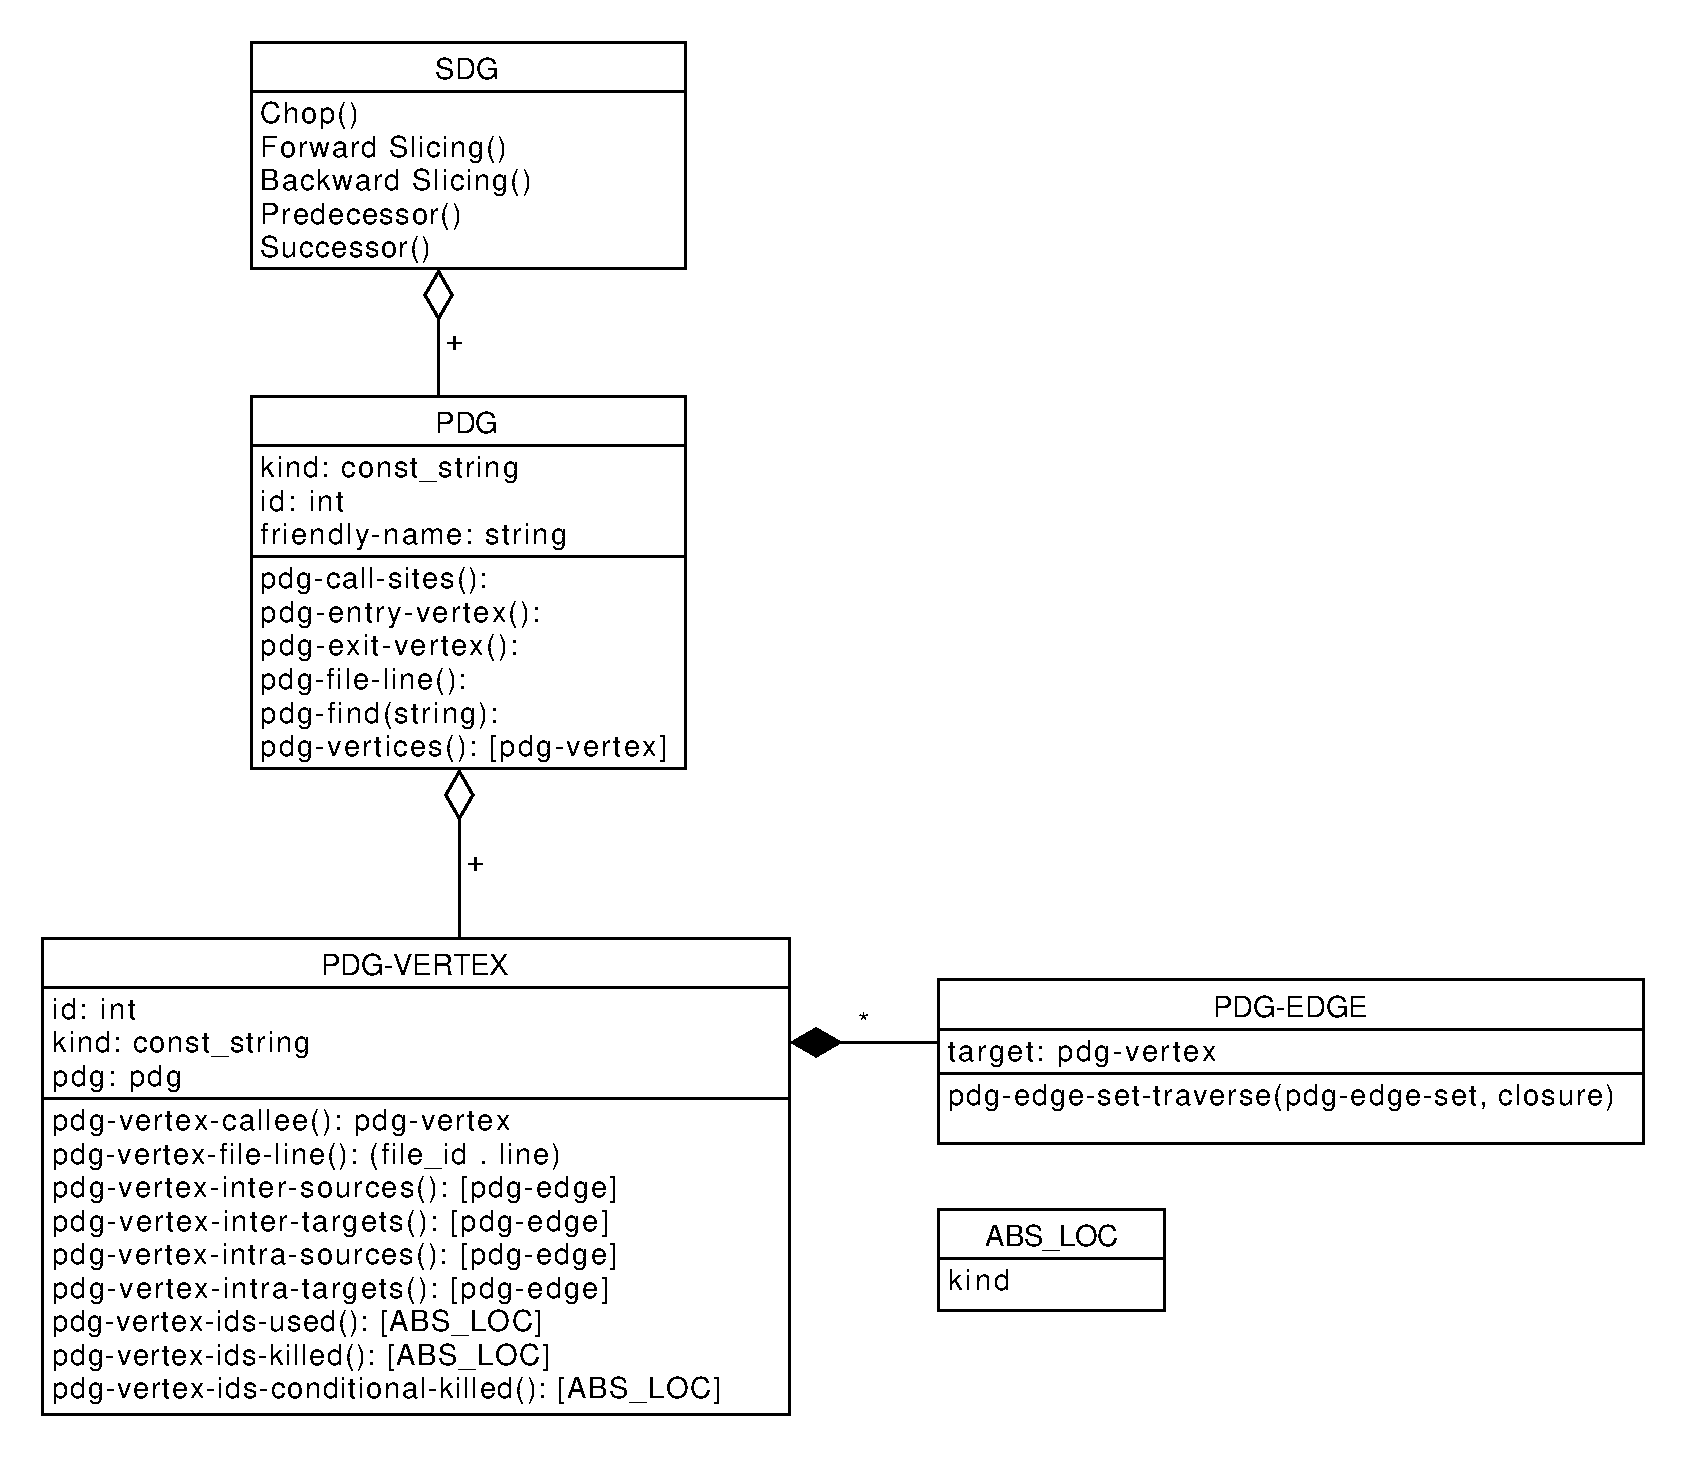
\includegraphics[ width=1.2 \linewidth]{./img/csurf_classdiagram.pdf}
	\caption{Code surfer data structure}
	\label{csurf_uml}
\end{figure}


\section{Data Distance}
The main point of distance graph can be summarized as follow: for a given pdg fin all its vertexes and for each vertex build a pair (used.killed) where:
\begin{itemize}
	\itembf{Used:} a program point where a variable is taken (i.e. read in some way). Can be used directly or indirectly is accessed using its pointer.
	
	\itembf{Killed:} a program point where the value contained in a variable is necessarily changed is a kill of that variable. A conditional kill is a kill bounded to a condition, so a c.k. may or may not happen.
\end{itemize}
Each couple represents a use-kill bound which is an edge in the graph, for example  $x = y +1$ corresponds to a pair (x.y).


\begin{figure}
	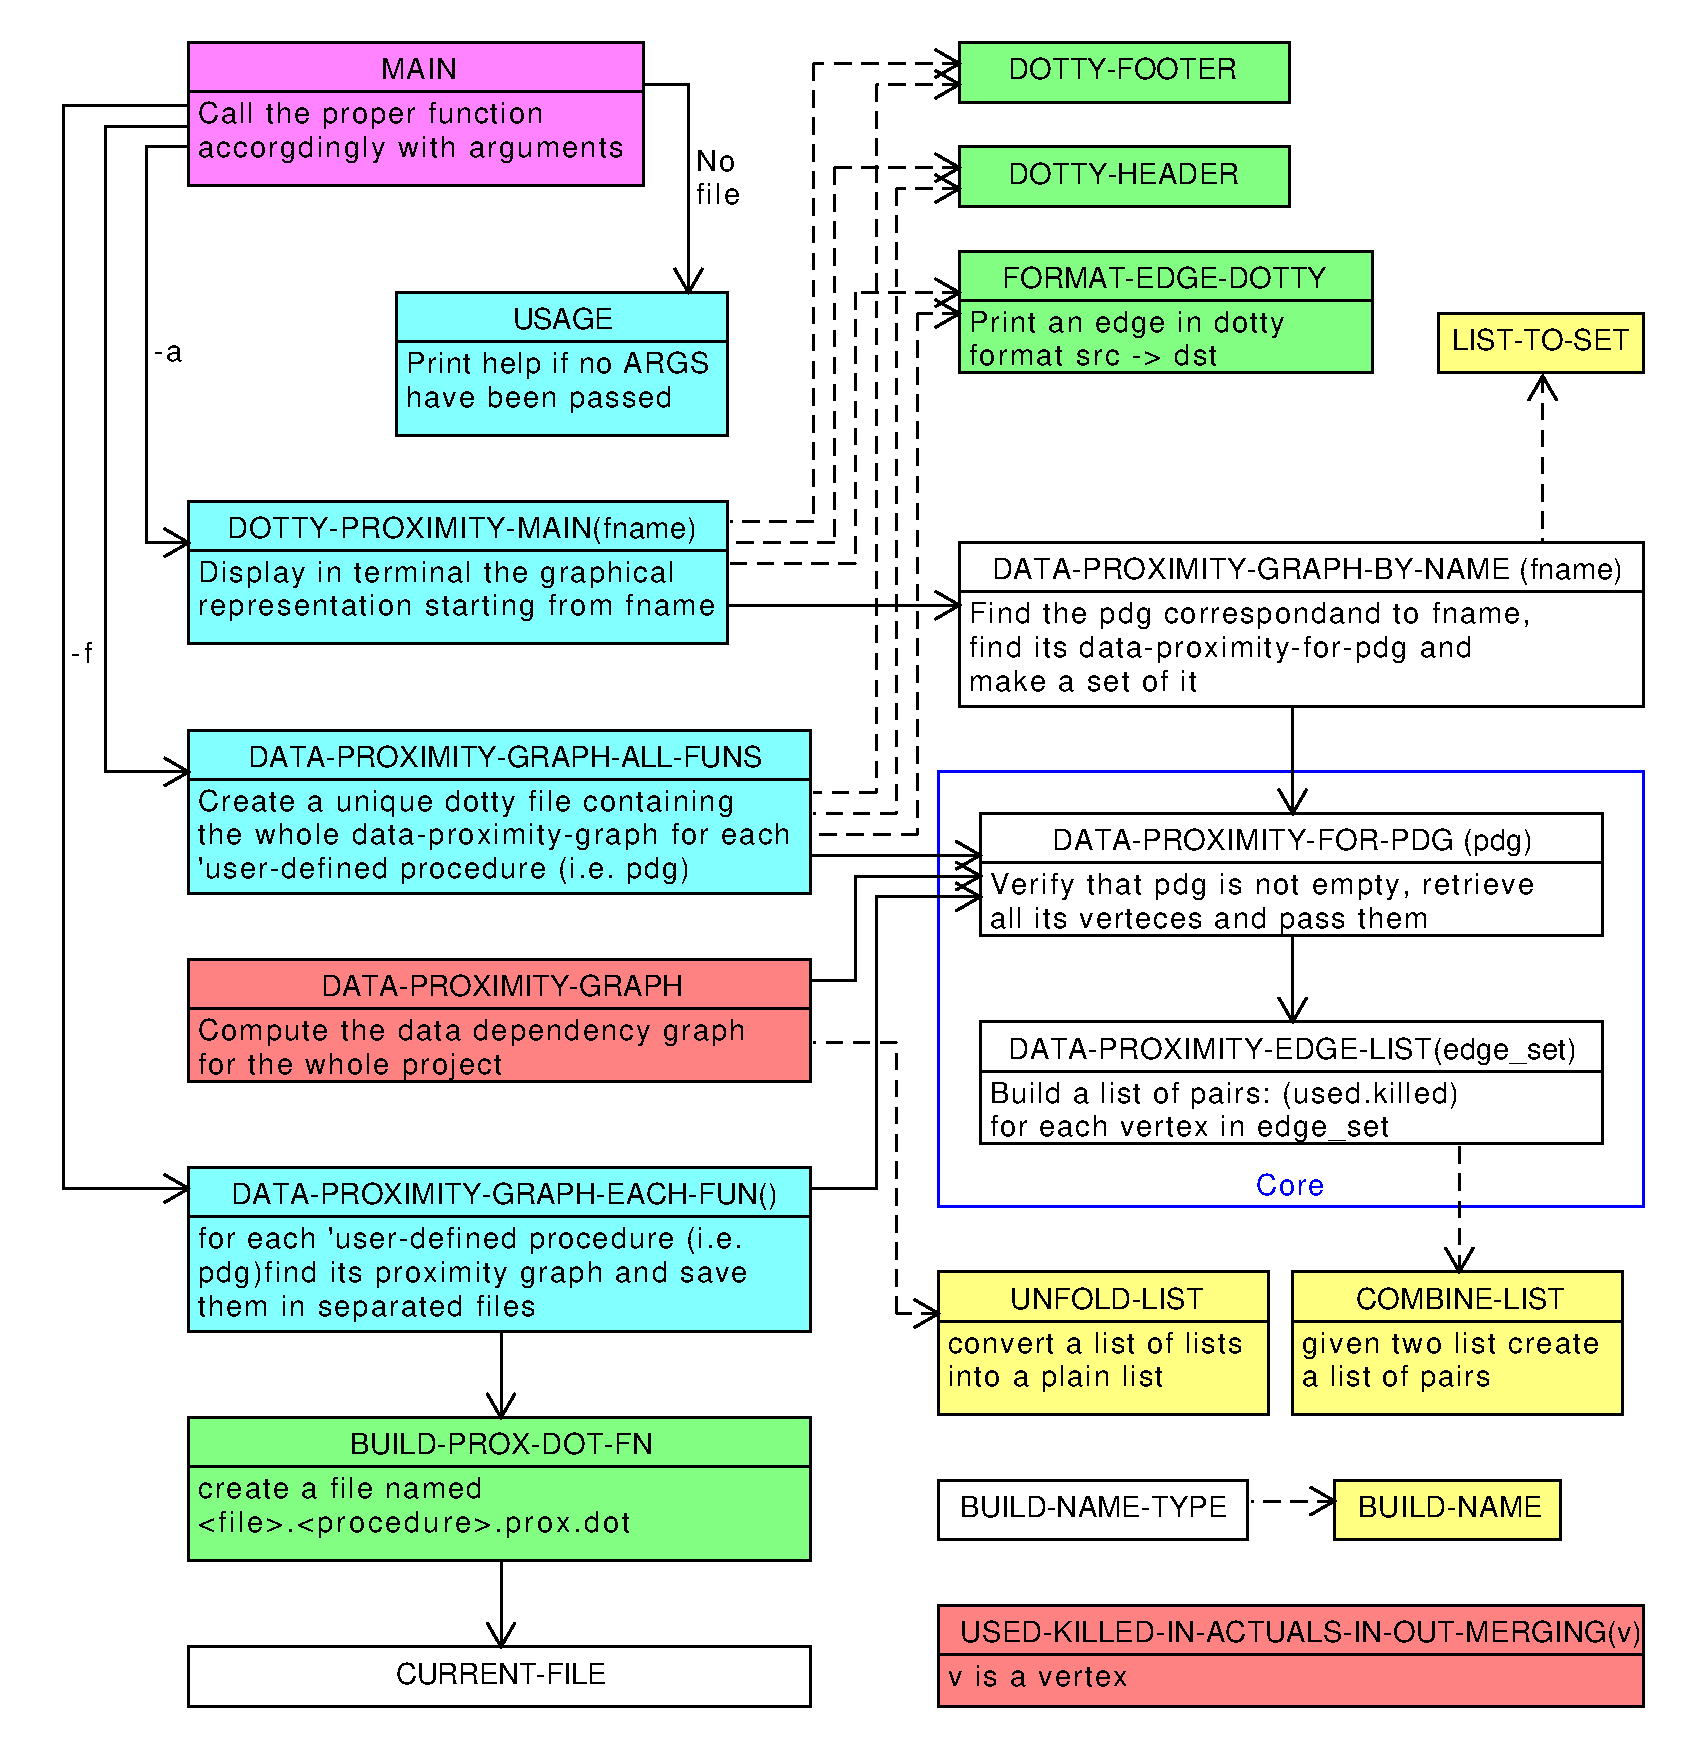
\includegraphics[ width=1 \linewidth]{./img/dd_descr_tree.pdf}
	\caption{Tiella's dd.stk program structure. Magenta represents main, cyan option args-dependent function, green output function (dotty support) and yellow are externally-defined functions.}
	\label{dd_uml}
\end{figure}


	
\bibliographystyle{ieeetr}
\bibliography{notex}

\end{document}
